%!TeX root=../tese.tex
%("dica" para o editor de texto: este arquivo é parte de um documento maior)
% para saber mais: https://tex.stackexchange.com/q/78101

\chapter{Metodologia de Pesquisa} 

\todo[inline]{Marília, é sempre bom ter um parágrafo inicial que dê uma visão geral sobre de que se trata o capítulo, para ele não começar direto em uma seção.} 

\section*{\textit{Design Science Research}}
% adiciona seção sem numeração ao sumário (toc)
\addcontentsline{toc}{section}{\textit{Design Science Research}}

A \textit{Design Science Research} (DSR) é uma metodologia de pesquisa utilizada na elaboração de artefatos com propósitos práticos, constituindo um processo de resolução de problemas de domínio, em que o resultado deve ser avaliado pelo seu valor e utilidade. Esse paradigma é aplicado em diferentes áreas de pesquisa, como Sistemas de Informação, Gerenciamento de Negócios, Engenharia de Software, etc, podendo ser instanciado em variantes muito diferentes \citep{dresch2015design, runeson2020design}.

\citet{hevner2004design} definiram sete diretrizes para a realização de DSR na área de Sistemas de Informação, que têm como princípio a construção e aplicação de um artefato para adquirir conhecimento sobre um problema de design e sua solução. Assim, uma pesquisa em \textit{Design Science} requer a criação de um artefato com propósito para tecnologia da informação e com caráter inovador (diretriz 1), o qual deve considerar a solução de um problema de negócio relevante (diretriz 2). Além disso, o seu design deve ser avaliado rigorosamente considerando sua utilidade, qualidade e eficácia (diretriz 3). O artefato também deve ser inovador, proporcionando contribuições claras e verificáveis para pesquisa (diretriz 4), e sua construção e avaliação devem ser feitas de forma rigorosa (diretriz 5). O processo de design do artefato deve ser conduzido como um processo de pesquisa de uma solução efetiva para um problema (diretriz 6). Por fim, os resultados da pesquisa em \textit{Design Science} devem ser comunicados de forma eficaz (diretriz 7).

%%%%%%%%%%%%%%%%%%%%%%%%%%%%%%%%%%%%%%%%%%%%%%%%%%%%%%%%%%%%%%%%%%%%%%%%%%%%%%%%
%%% Diretrizes Hevner (2004)
% \begin{enumerate}
%     \item \textbf{Design como um artefato:} criação de um artefato com propósito para TI e com caráter inovador
%     \item \textbf{Relevância do problema:} o artefato deve considerar a solução de um problema de negócios relevante
%     \item \textbf{Avaliação do design:} o design do artefato deve ser avaliado rigorosamente considerando sua utilidade, qualidade e eficácia
%     \item \textbf{Contribuições de pesquisa:} o artefato deve ser inovador, proporcionando contribuições claras e verificáveis para pesquisa
%     \item \textbf{Rigor de pesquisa:} a construção e avaliação do artefato projetado devem ser feitas de forma rigorosa
%     \item \textbf{Design como um processo de pesquisa:} o processo de design do artefato é um processo de pesquisa de uma solução efetiva para um problema
%     \item \textbf{Comunicação da pesquisa:} os resultados da pesquisa em Design Science devem ser comunicados de forma efetiva
% \end{enumerate}
%%%%%%%%%%%%%%%%%%%%%%%%%%%%%%%%%%%%%%%%%%%%%%%%%%%%%%%%%%%%%%%%%%%%%%%%%%%%%%%%

\citet{wieringa2014design} estendeu a definição de \textit{Design Science}, apresentando diretrizes para realizar pesquisas em Sistemas de Informação e Engenharia de Software. Para o autor, a interação entre o artefato e o contexto do problema contribui para chegar à solução do problema. Dessa forma, um projeto de DS itera sobre as atividades de design e investigação. A atividade de design é decomposta em três tarefas, designadas como ciclo de design. Este ciclo está inserido em um outro, de engenharia, no qual temos o resultado do ciclo de design sendo introduzido no contexto real e avaliado. As etapas de cada um dos ciclos estão descritas a seguir:

\noindent \textbf{Ciclo de Engenharia:}

\begin{itemize}
    \item \textbf{Ciclo de Design:}
    \begin{itemize}
        \item \textbf{Investigação do Problema:} qual problema deve ser investigado e por quê?
        \item \textbf{Design do Tratamento (\textit{Treatment Design}):} projeto de um ou mais artefatos para tratar o problema.
        \item \textbf{Validação do Tratamento (\textit{Treatment Validation}):} análise para validar se esse projeto contribui para o tratamento do problema, caso seja implementado.
    \end{itemize}
    \item \textbf{Implementação do Tratamento (\textit{Treatment Implementation}):} tratamento do problema com um dos artefatos projetados.
    \item \textbf{Avaliação da Implementação (\textit{Implementation Evaluation}):} avaliação do sucesso do tratamento. Ao final desta etapa, podemos ter uma nova iteração no ciclo de engenharia.
\end{itemize}

\noindent O autor também destaca que projetos de pesquisa em \textit{Design Science} estão relacionados apenas às três etapas do ciclo de design.

\citet{runeson2020design} define etapas similares a estas para o ciclo de engenharia, envolvendo a conceitualização do problema, o projeto da solução e a validação empírica. Os autores explicam que a \textit{Design Science} abrange duas dimensões principais: problema-solução e teoria-prática. Eles descrevem as atividades de pesquisa que são realizadas de forma iterativa através das duas dimensões, são elas:

\begin{itemize}
    \item \textbf{Conceitualização do problema:} descrição do problema
    \item \textbf{Design da solução:} mapeamento do problema para uma solução geral
    \item \textbf{Abstração:} identificação de decisões de design importantes para uma solução válida dentro de um escopo definido
    \item \textbf{Instanciação:} implementação do artefato em contexto
    \item \textbf{Validação empírica:} avaliação de como a solução implementada abordou o problema
\end{itemize}

Ademais, projetos de pesquisa em \textit{Design Science} devem considerar dois fatores importantes: a relevância da pesquisa para entidades na resolução de problemas reais e o rigor para que a pesquisa seja considerada válida e confiável, contribuindo para uma determinada área. Dessa forma, a DSR é importante tanto para a produção de conhecimento científico como para a resolução de problemas reais \citep{dresch2015design, runeson2020design}.

Portanto, a \textit{Design Science} aborda problemas gerais através do estudo de instâncias específicas de problemas no contexto de pesquisa. Para realizar este projeto, seguimos a metodologia de \textit{Design Science Research} em Engenharia de Software proposta por \citet{wieringa2014design}, englobando o ciclo de design e de engenharia. Nas seções a seguir, descrevemos as etapas de cada ciclo referentes a esta pesquisa.

\section{Ciclo de Design}

\subsection{Investigação do Problema}
% Qual problema deve ser investigado e por quê?

O problema investigado neste estudo foi o de uso de simulações interativas no ensino de conceitos de lógica de programação para crianças. Como apresentado no Capítulo~\ref{related_tools}, diferentes metodologias são adotadas para isso, utilizando recursos didáticos variados, sendo as linguagens visuais as mais utilizadas. Dessa maneira, investigamos o uso de simulações interativas para o ensino de computação, uma vez que elas podem facilitar a visualização de ideias abstratas envolvidas nos conceitos de programação, utilizando exemplos concretos para representá-las. Ademais, essa metodologia se mostrou eficaz em outras ciências, com o uso da ferramenta PhET. Portanto, queremos expandi-la e testá-la em outros ambientes de aprendizado, como na área de Ciência da Computação.

%%%%%%%%%%%%%%%%%%%%%%%%%%%%%%%%%%%%%%%%%%%%%%%%%%%%%%%%%%%%%%%%%%%%%%%%%%%%%%%%
% Problema?
% - representações visuais dos conceitos de lógica de programação para o ensino de computação para crianças
% - nova abordagem para ensino dos conceitos de lógica de programação para crianças
%
% Etapas
% - estudo sobre o ensino de computação para crianças
% - busca extensiva de ferramentas de apoio pedagógico existentes
%%%%%%%%%%%%%%%%%%%%%%%%%%%%%%%%%%%%%%%%%%%%%%%%%%%%%%%%%%%%%%%%%%%%%%%%%%%%%%%%

Para investigar o problema, primeiramente, realizamos uma pesquisa sobre o estado atual do ensino de computação para crianças em escolas no Brasil e no mundo. Em seguida, fizemos uma busca extensiva dos diversos tipos de ferramentas de apoio pedagógico existentes e similares a proposta neste trabalho, procurando entender as principais diferenças entre elas. Grande parte dessa pesquisa foi realizada durante o desenvolvimento do projeto de Iniciação Científica (IC) intitulado \enquote{Uma Ferramenta de Simulações Interativas para Ensino de Computação para Crianças}, realizado entre outubro de 2022 e outubro de 2023. O resumo dos principais resultados dessa investigação se encontra nos Capítulos \ref{introduction} e \ref{related_tools} desta monografia.

%%%%%%%%%%%%%%%%%%%%%%%%%%%%%%%%%%%%%%%%%%%%%%%%%%%%%%%%%%%%%%%%%%%%%%%%%%%%%%%%
% A seguir, com as demais etapas do ciclo de design e engenharia veremos, então, como as simulações de conceitos de lógica de programação podem ser ferramentas de aprendizado eficazes no ensino de computação para crianças.
%%%%%%%%%%%%%%%%%%%%%%%%%%%%%%%%%%%%%%%%%%%%%%%%%%%%%%%%%%%%%%%%%%%%%%%%%%%%%%%%

\subsection{Projeto do Artefato} \label{design}
% projeto de um ou mais artefatos para tratar o problema.

O artefato projetado como tratamento do problema é um MVP de uma ferramenta de simulações interativas de conceitos de lógica de programação destinada a crianças do ensino fundamental. Um MVP (\textit{Minimum Viable Product}) ou produto mínimo viável é um produto com funcionalidades suficientes para ser utilizado por usuários iniciais que possam fornecer \textit{feedback} com o intuito de validar uma ideia. 

No ensino da computação, alguns conceitos introdutórios são fundamentais para o aprendizado da lógica de programação, tais como variáveis, entrada e saída, operadores lógicos e aritméticos, condicionais, laços de repetição, funções, vetores, matrizes, entre outros. Desse modo, para testar a viabilidade do protótipo proposto, seu projeto deve compreender um conjunto mínimo desses conceitos, a fim de verificar o entendimento deles pelos usuários. 

Assim, para projetar os artefatos ou protótipos do MVP, primeiramente, definimos alguns requisitos mínimos, listados a seguir:

\begin{itemize}
    \item O MVP deve apresentar uma tela com uma área de trabalho e uma opção de ajuda com uma documentação explicativa de uso;
    \item A área de trabalho deve apresentar um espaço fixo para a simulação e outro para o pseudocódigo correspondente;
    \item A simulação deve envolver os seguintes conceitos de lógica de programação: variáveis, entrada, operadores (aritméticos, lógicos e de comparação), condicionais e laços de repetição;
    \item A simulação deve apresentar um número limitado de interações possíveis com o usuário;
    \item A simulação deve encorajar os usuários a explorá-la livremente, com controles intuitivos e uma interface que possibilite boa usabilidade;
    \item O pseudocódigo deve ser gerado automaticamente conforme as interações com a simulação vão ocorrendo.
\end{itemize}

Além disso, também definimos e descrevemos os conceitos de lógica de programação que foram simulados e a sintaxe do pseudocódigo gerado. A partir dos protótipos iniciais, estudamos ideias similares e validamos os artefatos projetados para analisar alterações necessárias e as melhores opções de implementação. O Capítulo \ref{prototypes} apresenta em detalhes o desenvolvimento dos protótipos propostos.

%%%%%%%%%%%%%%%%%%%%%%%%%%%%%%%%%%%%%%%%%%%%%%%%%%%%%%%%%%%%%%%%%%%%%%%%%%%%%%%%
% Para isso, dois protótipos iniciais de simulações a serem desenvolvidas foram desenhados no Figma\footnote{\url{https://www.figma.com/}}, uma plataforma web colaborativa para projetar interfaces. As Figuras~\ref{figure:brinquedos1} e~\ref{figure:festa1} mostram esses protótipos.

% \begin{figure}[h!]
%     \centering
%     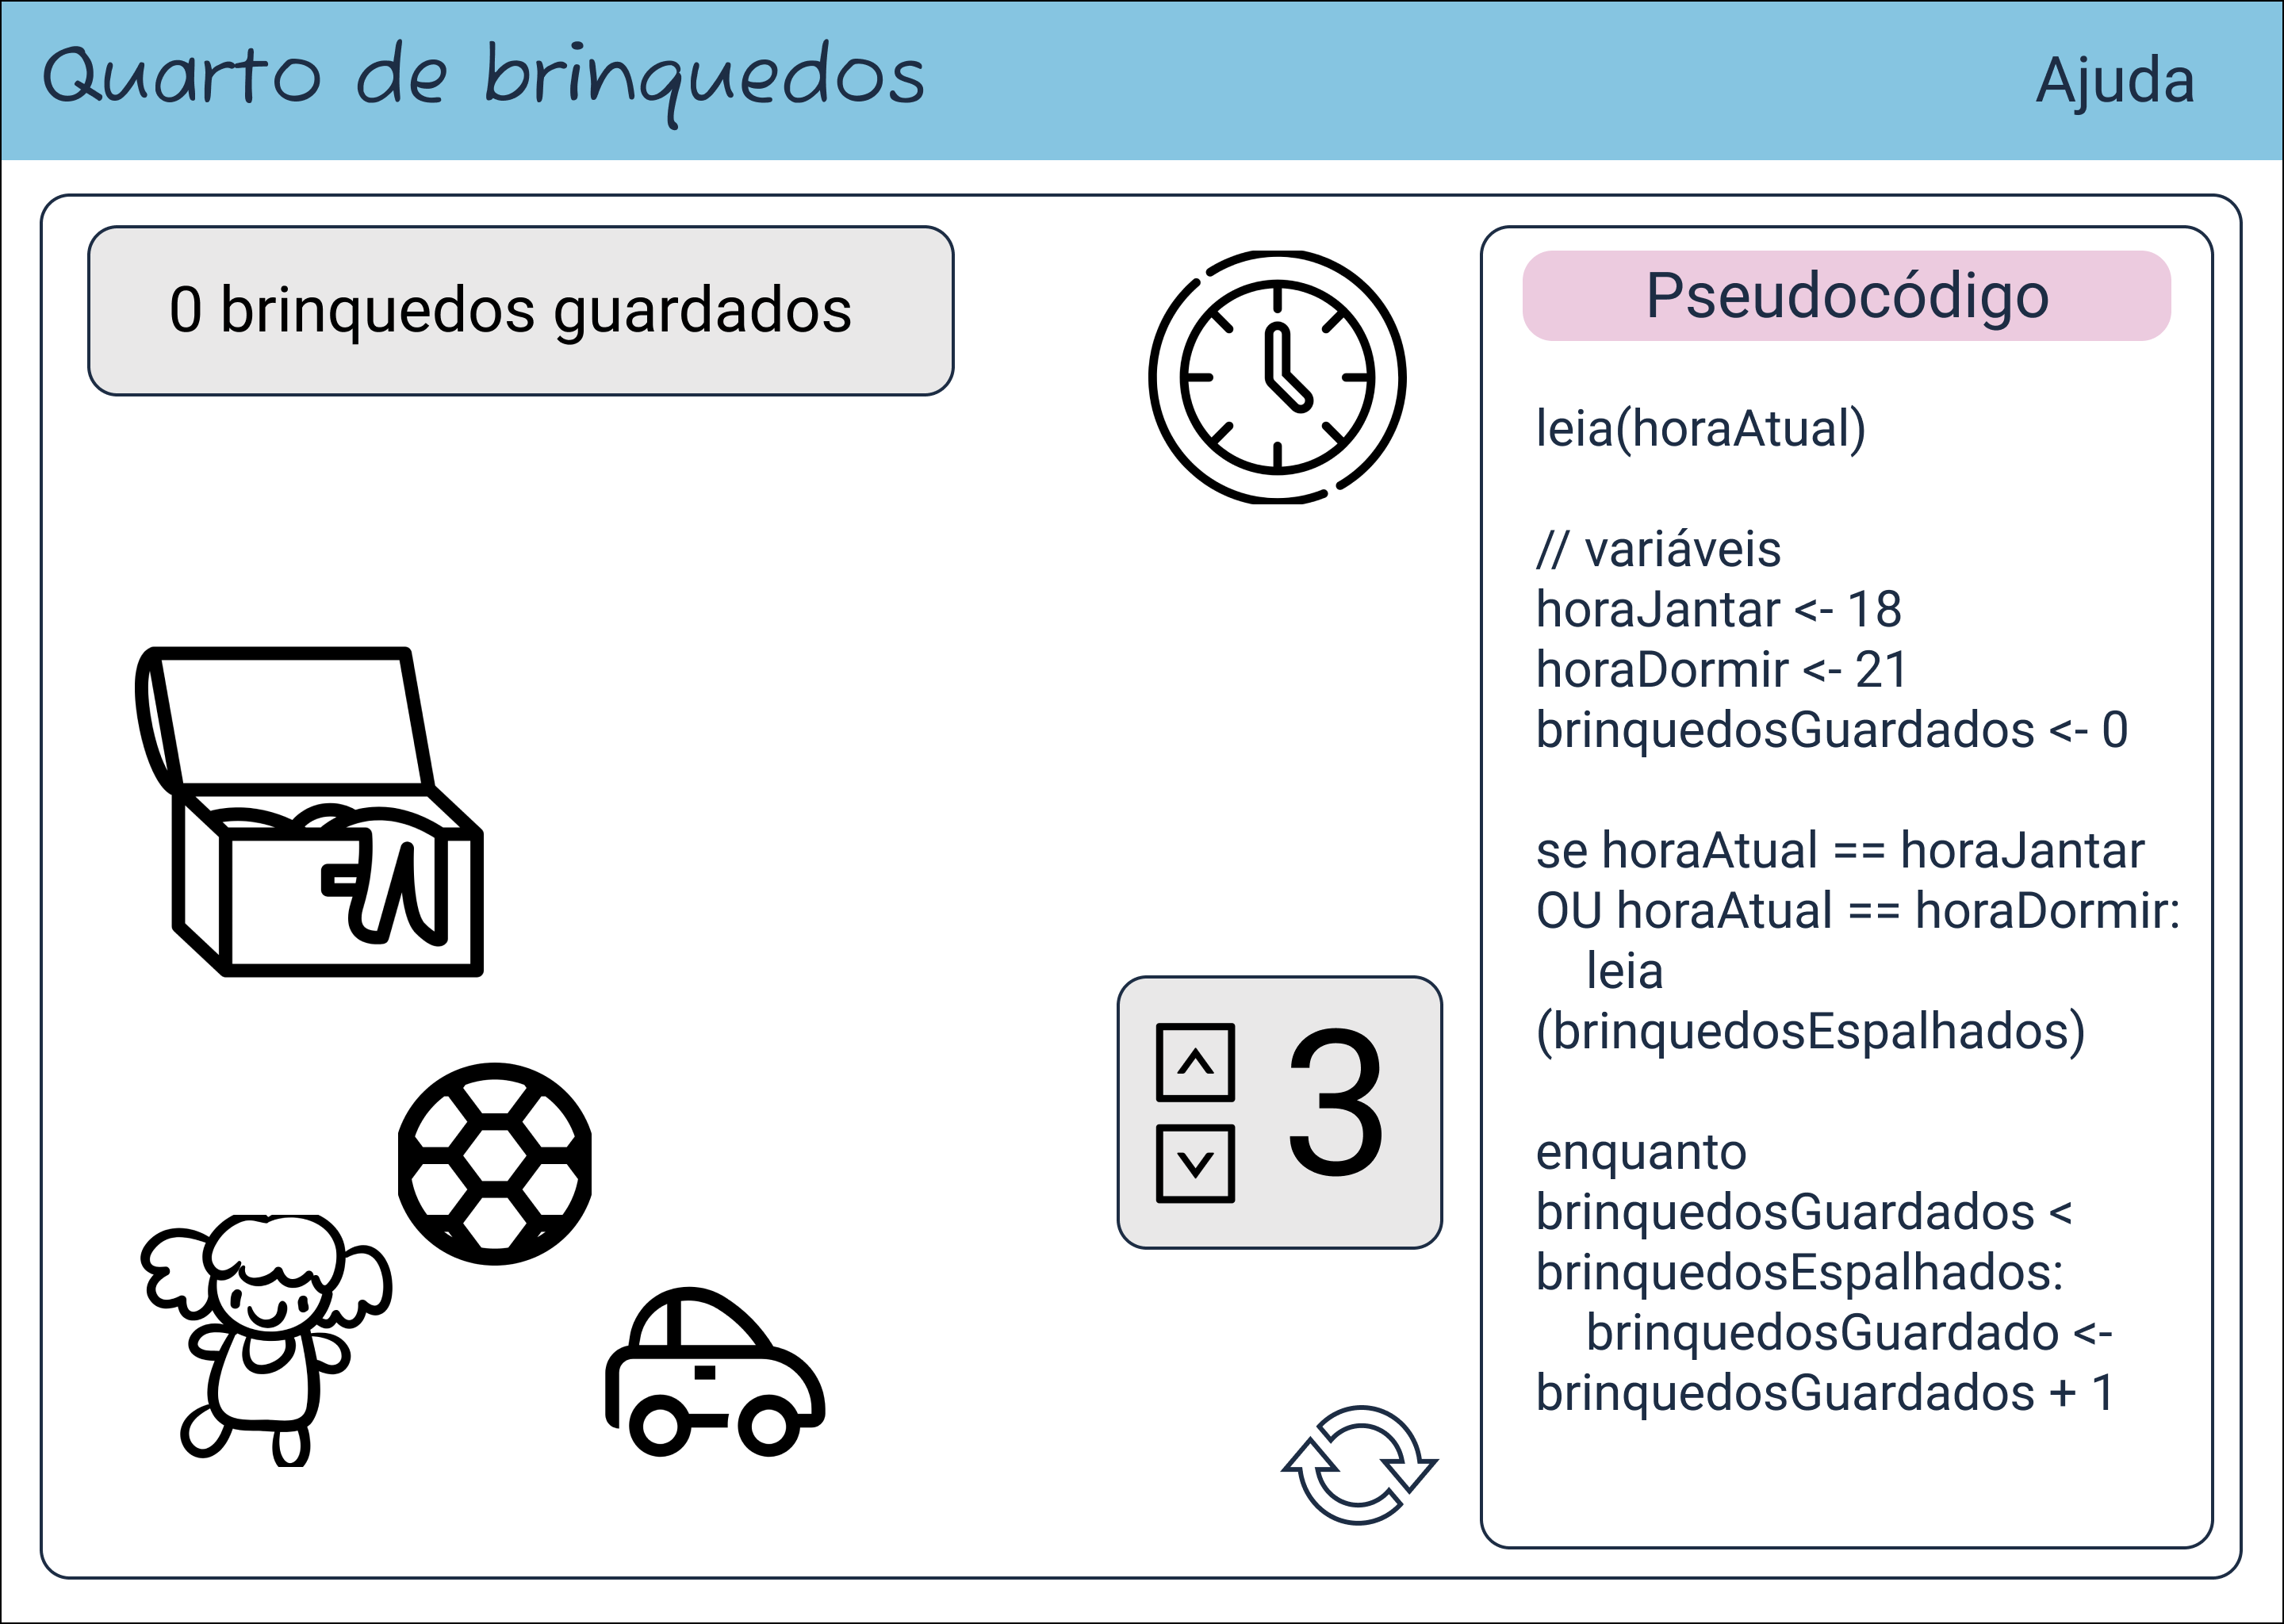
\includegraphics[scale=0.15]{prototipo_brinquedos1.png}
%     \caption{Protótipo inicial da simulação \enquote{Quarto de Brinquedos}.}
%     \label{figure:brinquedos1}
% \end{figure}

% \begin{figure}[h!]
%     \centering
%     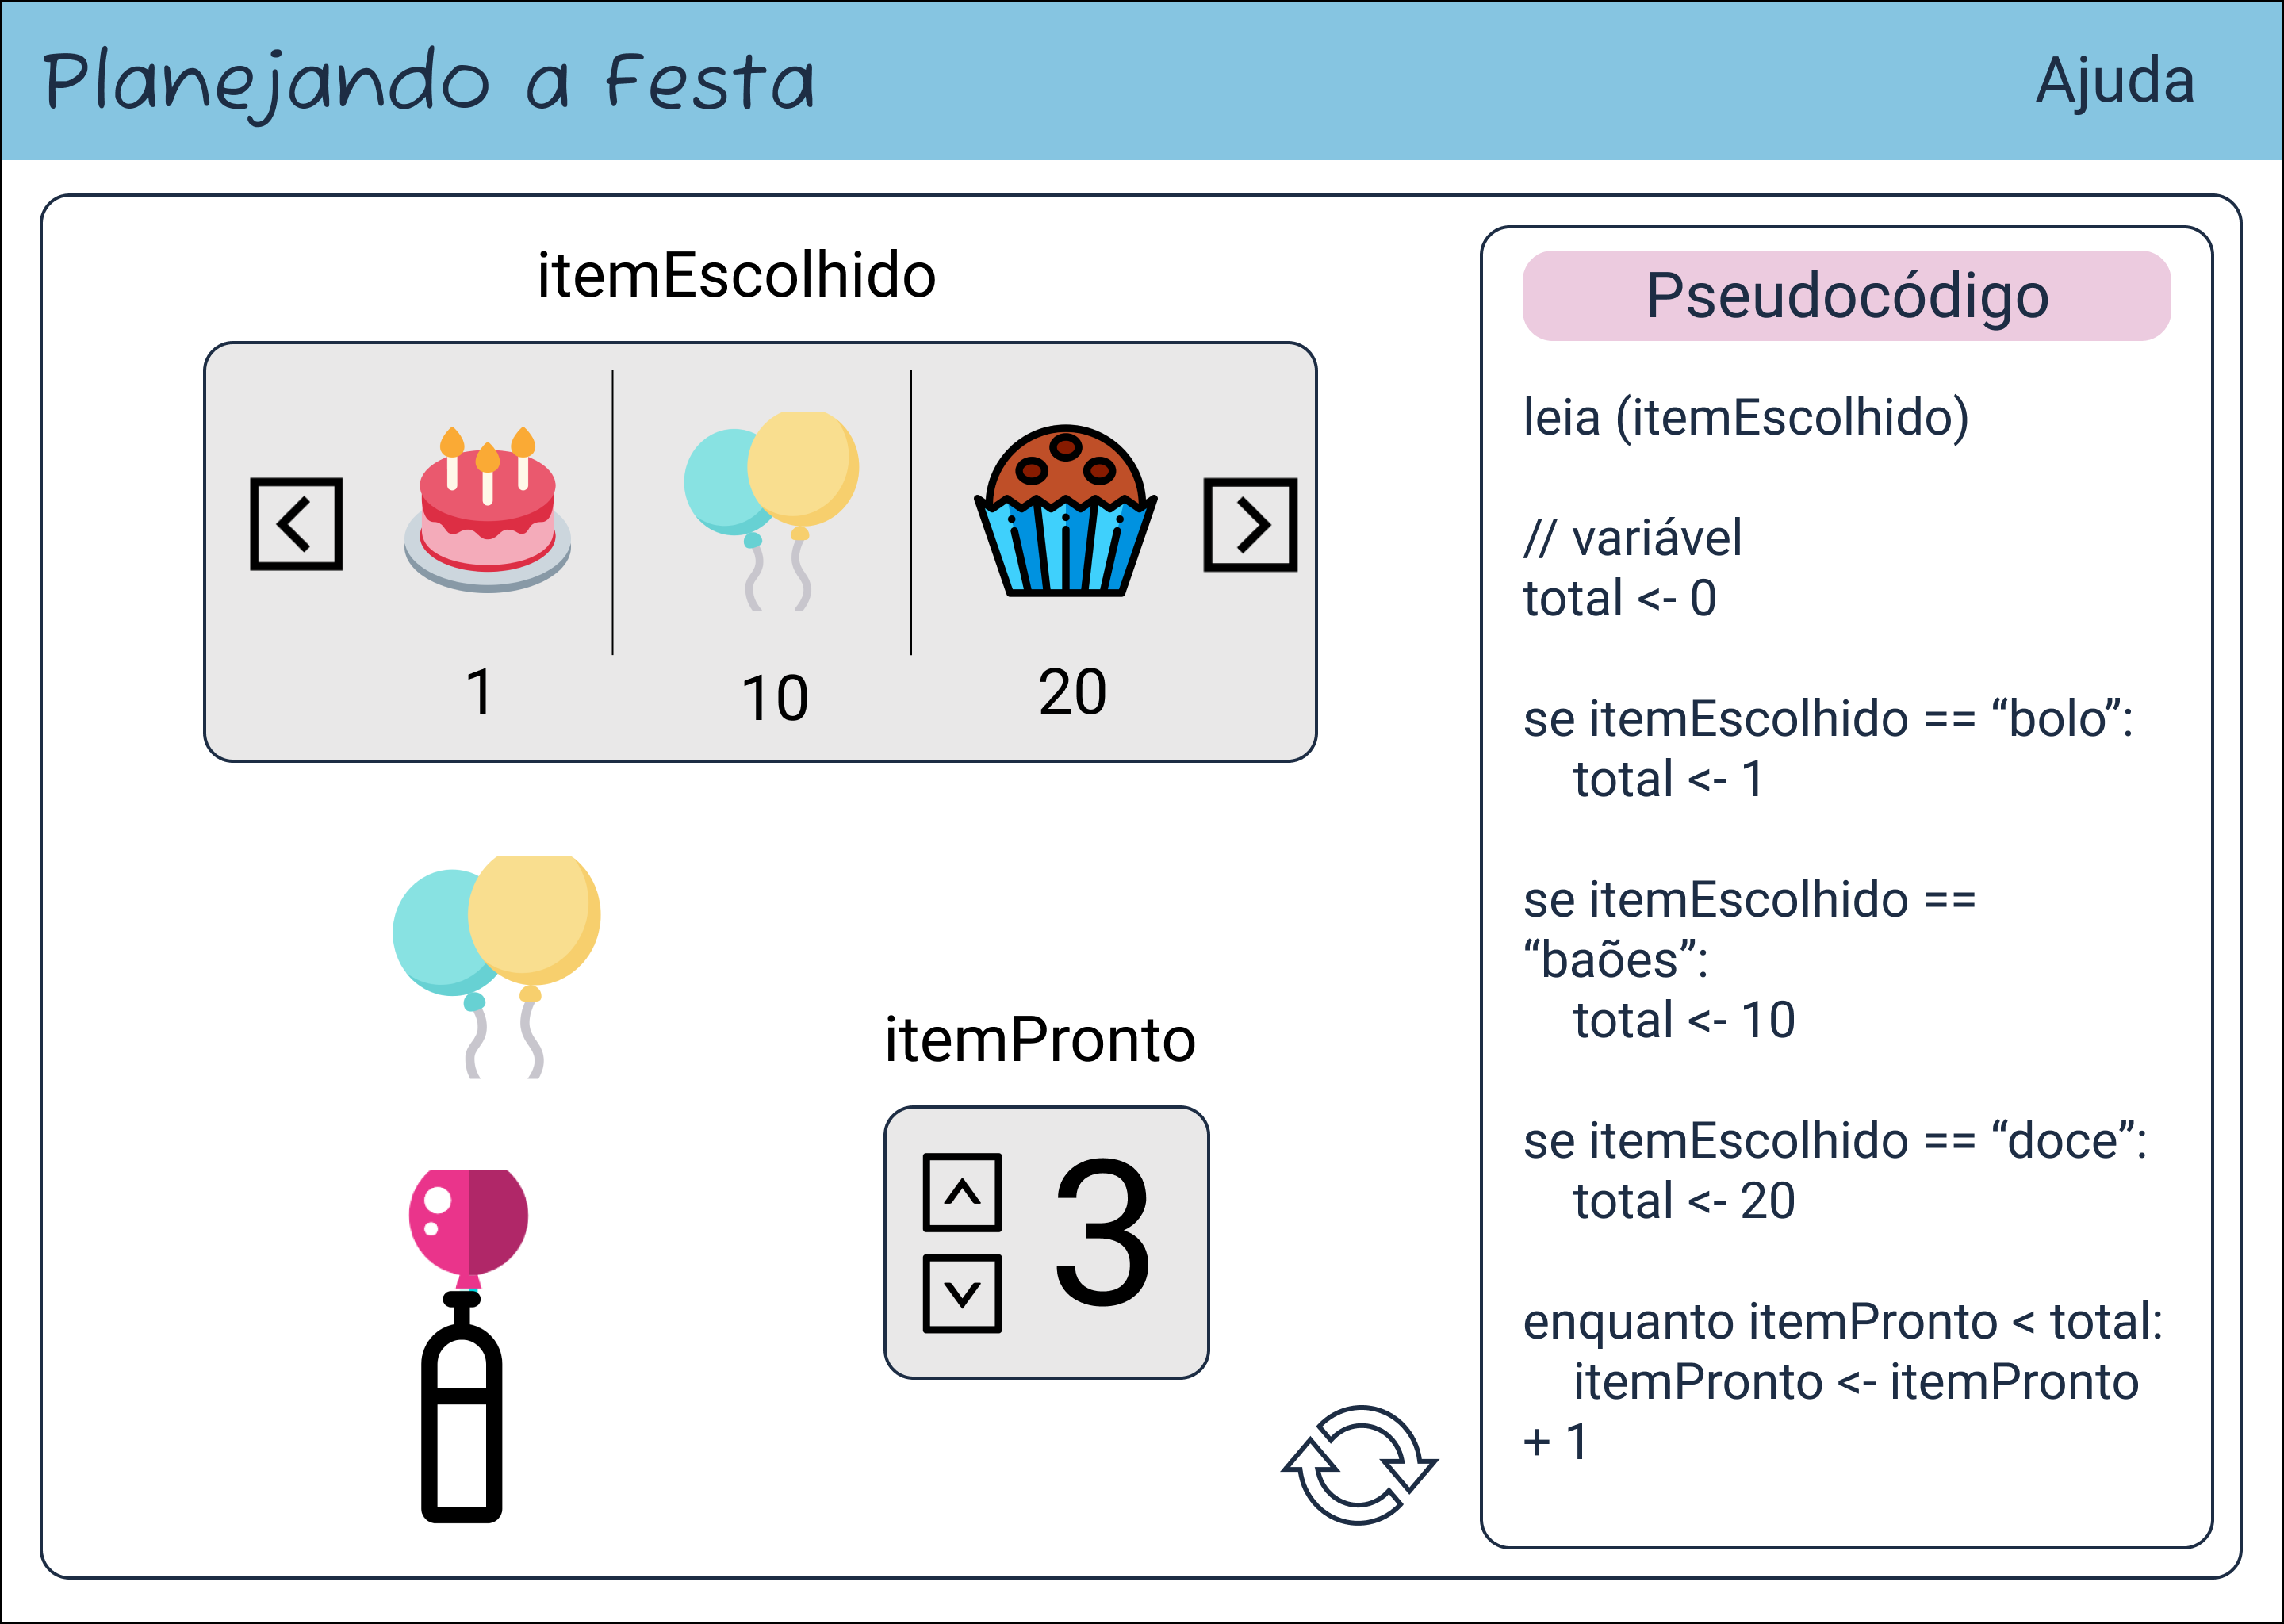
\includegraphics[scale=0.15]{prototipo_festa1.png}
%     \caption{Protótipo inicial da simulação \enquote{Planejando a Festa}.}
%     \label{figure:festa1}
% \end{figure}

% Na Figura \ref{figure:brinquedos1}, temos um cenário de quarto de brinquedos. O protótipo da simulação apresenta elementos visuais como um relógio de parede, um baú para guardar objetos e brinquedos espalhados pelo chão. Além disso, temos dois painéis, um controle para regular a quantidade de brinquedos espalhados e um contador que mostra quantos brinquedos foram guardados. Ainda, o protótipo apresenta um pseudocódigo associado à simulação.

% A princípio, a ideia desta simulação é apresentar duas interações possíveis: alterar a hora no relógio e guardar os brinquedos no baú de forma iterativa. Com isso, queremos abordar o conceito de variáveis, principalmente, com a ação de guardar os objetos em um contêiner; de entrada, com a informação recebida através da interação com o usuário ao alterar o horário; de operadores, na comparação de expressões simples e complexas com conectivos lógicos, e na operação de adição contida na ação de guardar os brinquedos; de condicionais, verificando se é o momento de organizar o quarto; e de laços de repetição, repetindo a ação de guardar cada objeto até que o quarto esteja organizado.

% A Figura \ref{figure:festa1} apresenta um cenário de planejamento de uma festa. Nele há elementos visuais que representam itens que podem ser escolhidos para incorporar uma festa de aniversário. Ademais, temos um contador que mostra quantos itens referentes ao escolhido já estão preparados. Nesta simulação, o usuário poderá ter duas interações: escolher um item para a festa e \enquote{prepará-lo} (incrementar um determinado item) até estar completo. Deste modo, neste cenário, abordamos os conceitos de variáveis, por meio do total de objetos que devemos ter de acordo com a escolha do item; de entrada, a partir da escolha de um item para a festa; de operadores, na comparação de expressões simples, e na operação de adição contida na ação de preparar um item; de condicionais, verificando qual item foi escolhido; e de laços de repetição, conforme incremento dos objetos até atingirem o total de acordo com cada elemento.
%%%%%%%%%%%%%%%%%%%%%%%%%%%%%%%%%%%%%%%%%%%%%%%%%%%%%%%%%%%%%%%%%%%%%%%%%%%%%%%%

\subsection{Validação do Artefato} \label{validation}
% análise para validar se esse projeto contribui para o tratamento do problema, caso seja implementado
A validação dos artefatos foi realizada com base nas opiniões de profissionais de ensino de computação e matemática. Foram consultados: a professora Dra. Kelly Braghetto do Departamento de Ciência da Computação do IME, minha orientadora no Trabalho de Formatura, que também coordena o projeto CodificADAs USP, oferecendo cursos introdutórios de programação voltados para meninas do ensino médio; a estudante Victoria Nóvoa, do curso de Licenciatura em Educomunicação da USP, instrutora de tecnologia educacional de crianças no Colégio Santa Cruz; e o professor Henri Silva da Escola de Aplicação da Faculdade de Educação da USP, que leciona matemática para alunos do 8° ano do Ensino Fundamental II.

Em conversas com os avaliadores, foi possível obter \textit{feedbacks} para verificar a usabilidade e utilidade do MVP a partir dos protótipos projetados, possibilitando o refinamento deles e a escolha de um artefato para implementação, além da definição do público alvo específico para testar a aplicação. No Capítulo \ref{prototypes}, descrevemos o processo de validação e as alterações realizadas. 

%%%%%%%%%%%%%%%%%%%%%%%%%%%%%%%%%%%%%%%%%%%%%%%%%%%%%%%%%%%%%%%%%%%%%%%%%%%%%%%%
% Primeiramente, antes de apresentarmos os artefatos para validação, realizamos alguns mudanças nos protótipos iniciais, conforme sugestões da professora Kelly. As Figuras \ref{figure:brinquedos2} e \ref{figure:festa2} mostram as alterações sugeridas para os artefatos.

% \begin{figure}[h!]
%     \centering
%     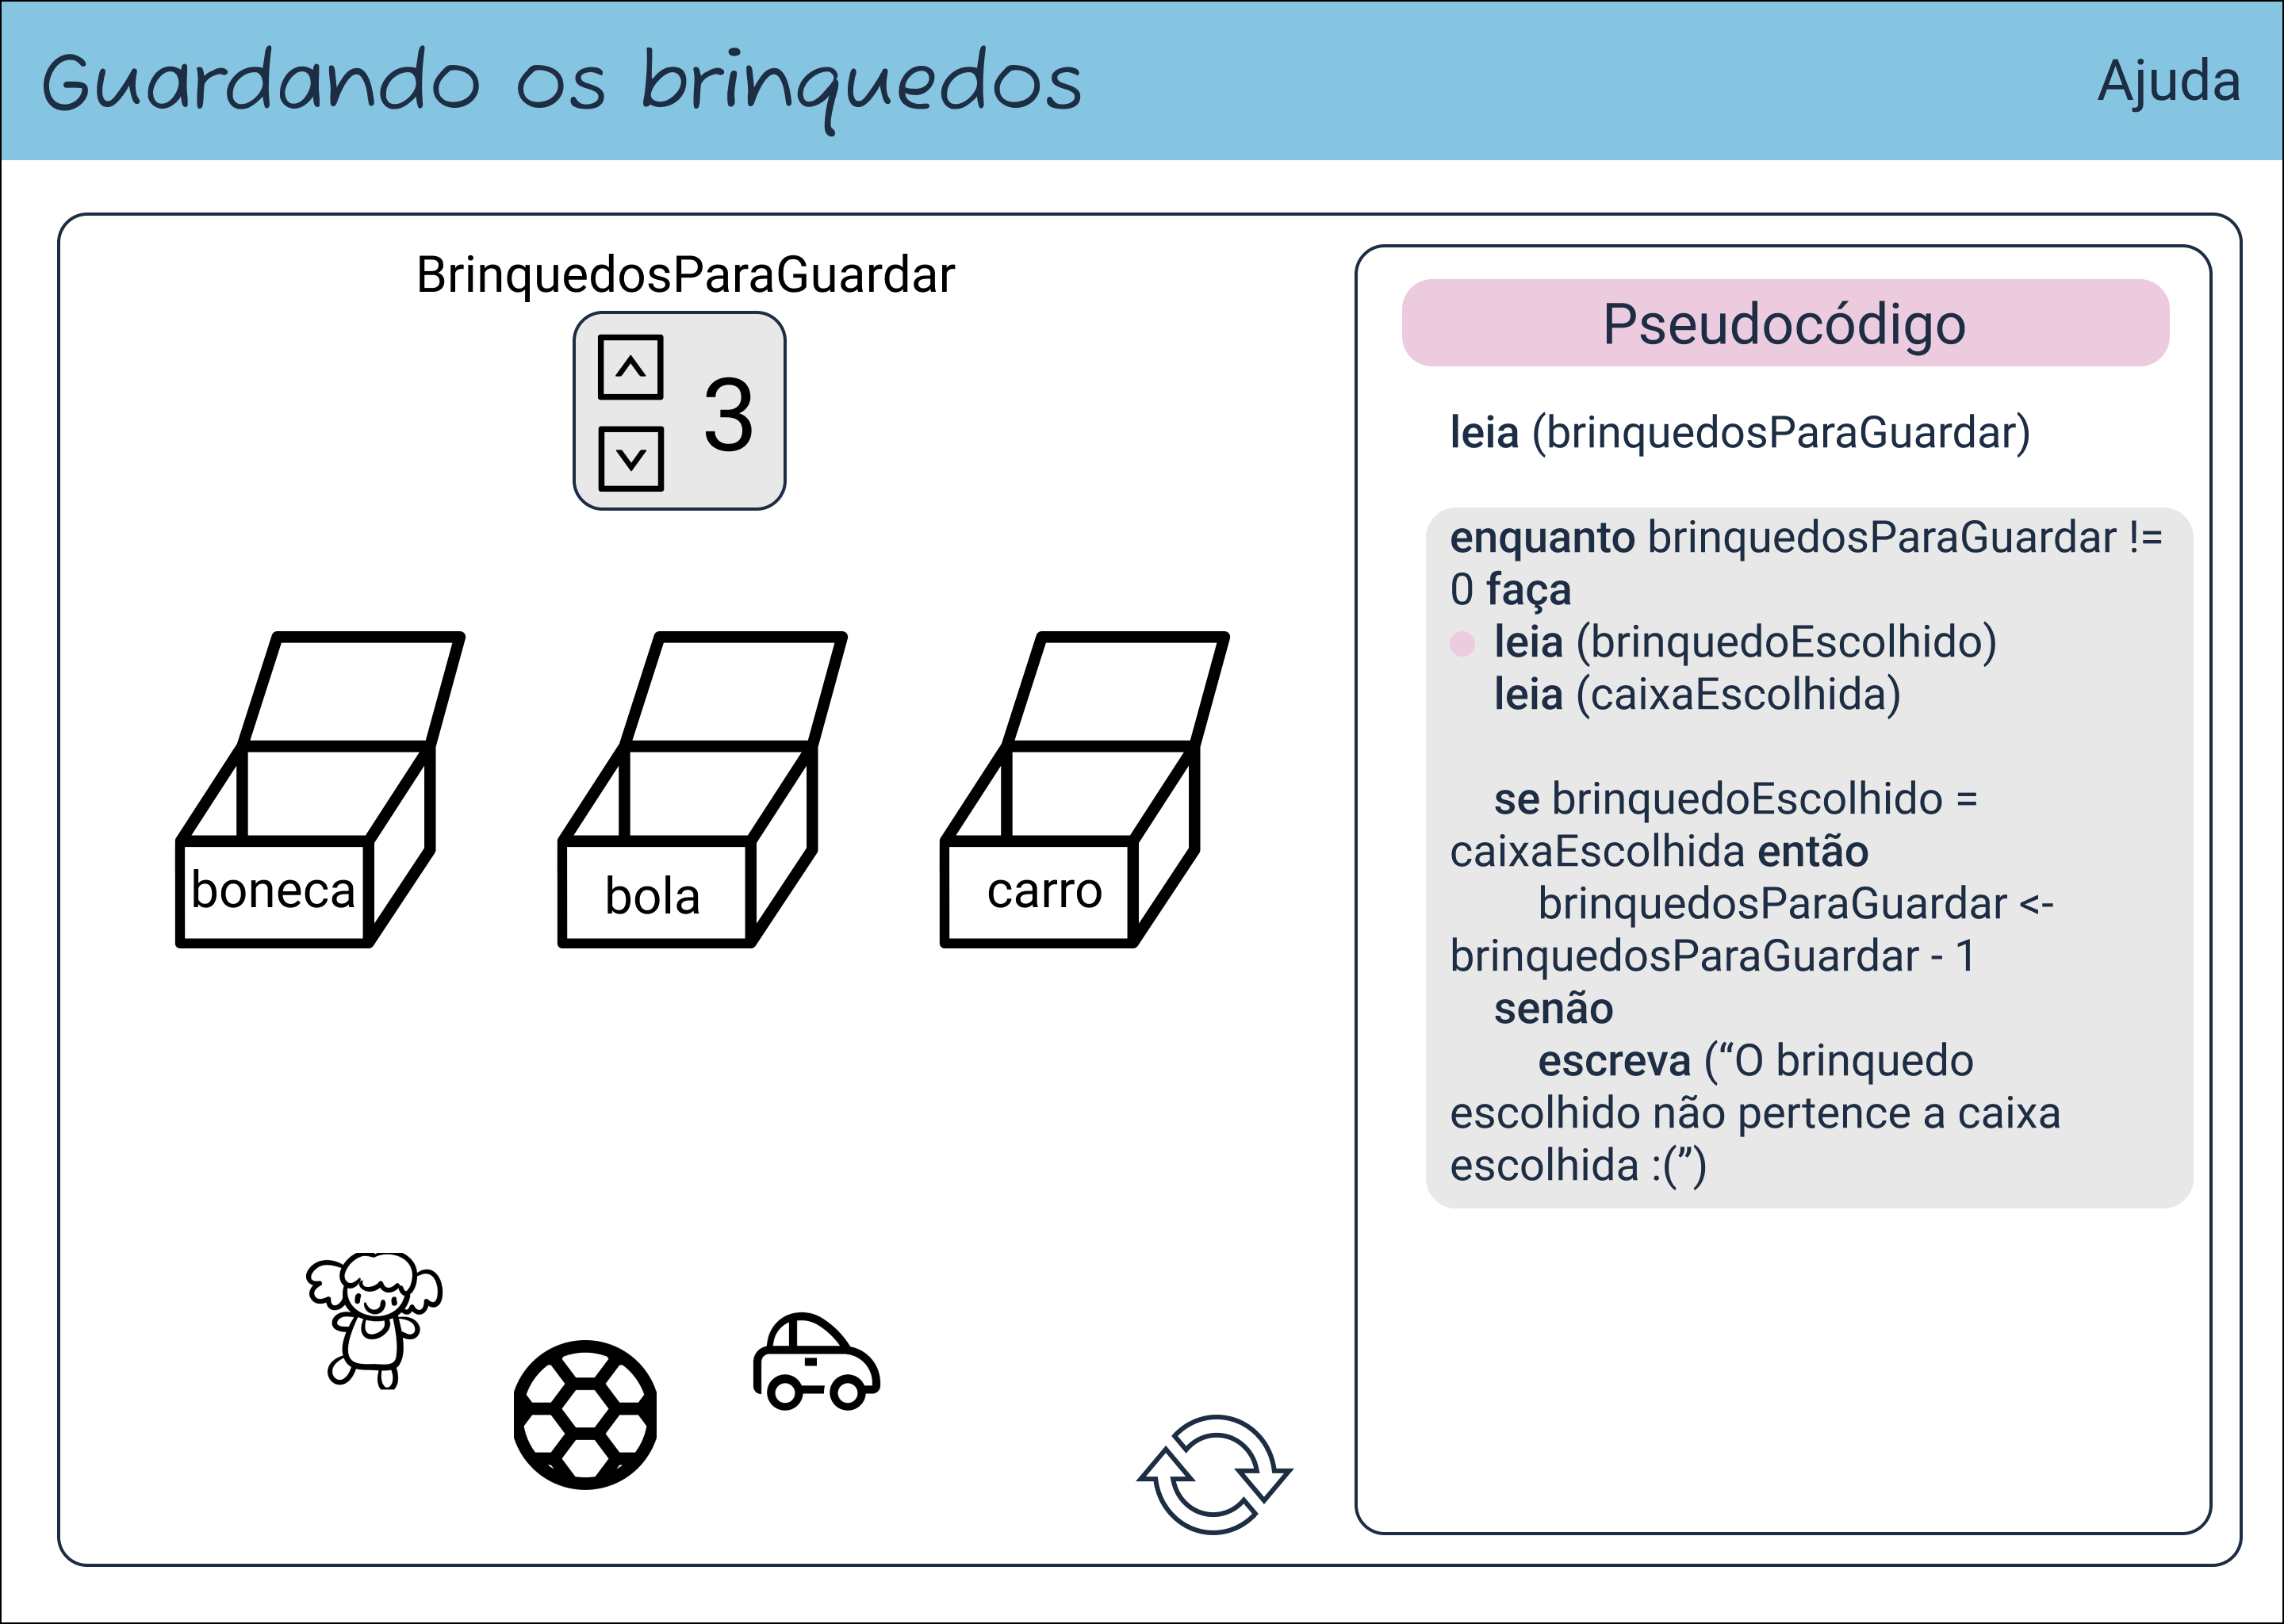
\includegraphics[scale=0.15]{prototipo_brinquedos2.png}
%     \caption{Protótipo da simulação \enquote{Guardando os Brinquedos} após validação.}
%     \label{figure:brinquedos2}
% \end{figure}

% \begin{figure}[h!]
%     \centering
%     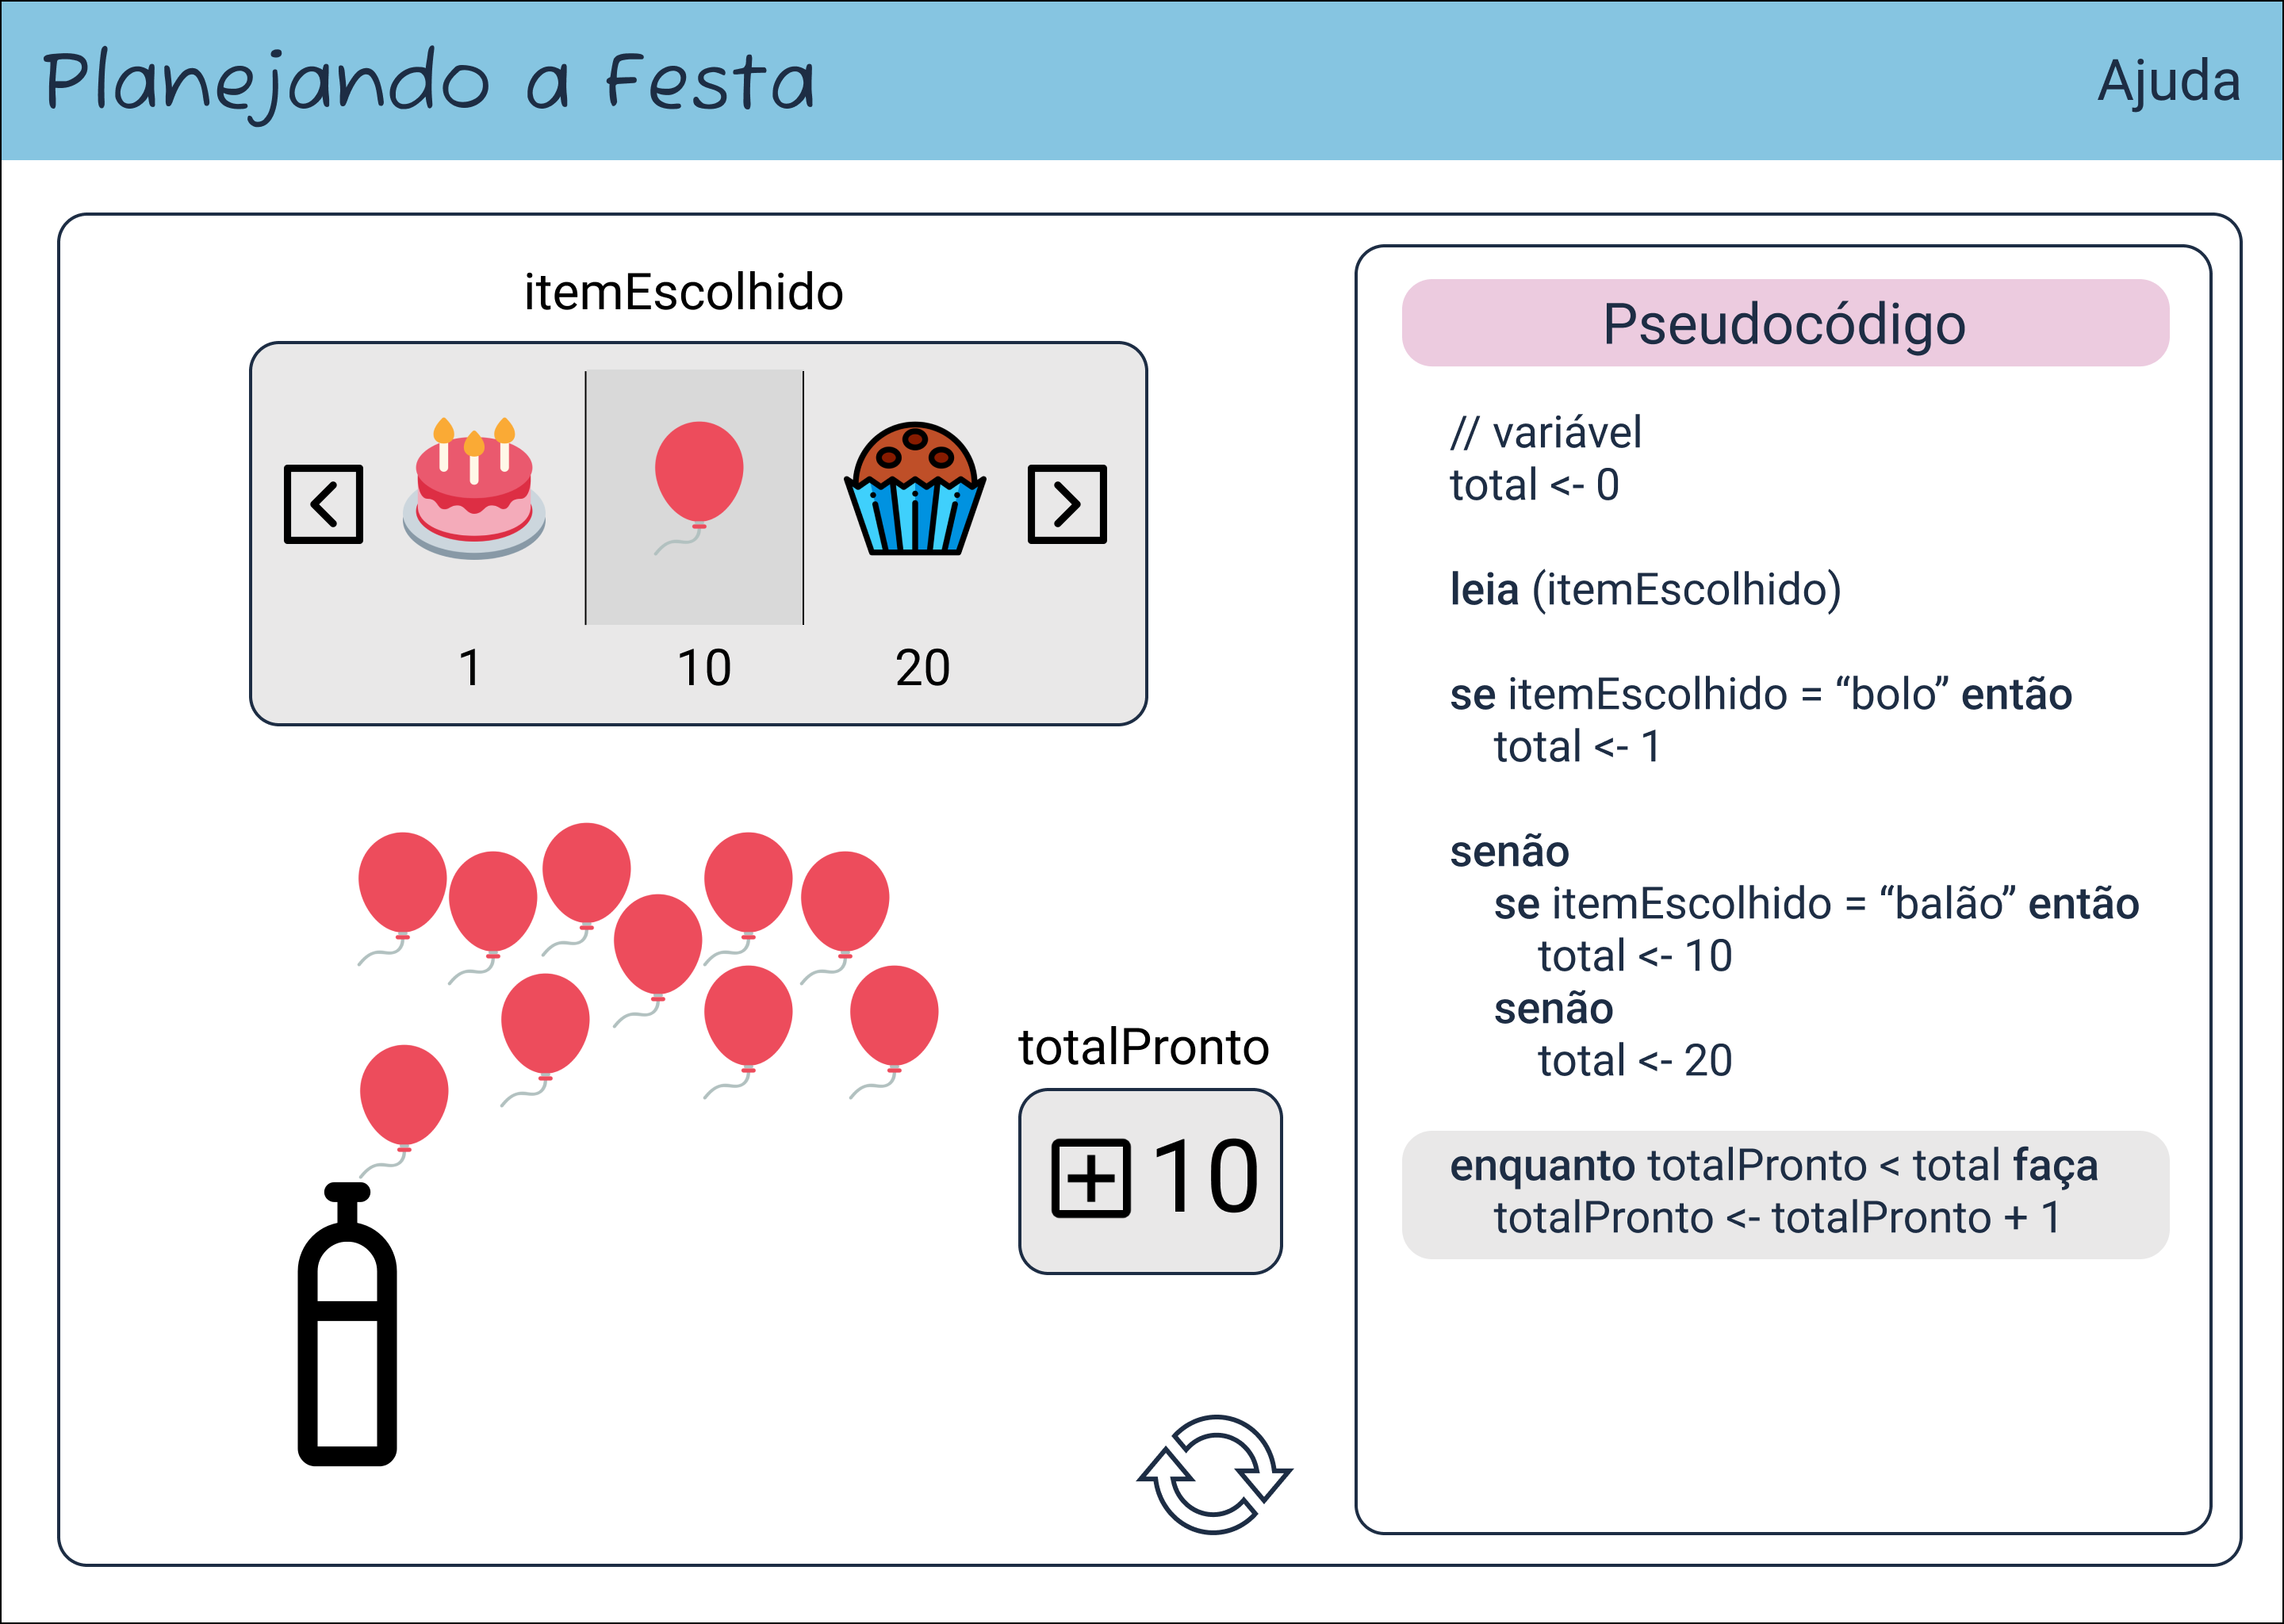
\includegraphics[scale=0.15]{prototipo_festa2.png}
%     \caption{Protótipo da simulação \enquote{Planejando a Festa} após validação.}
%     \label{figure:festa2}
% \end{figure}

% Na Figura \ref{figure:brinquedos2} podemos observar a nova simulação \enquote{Guardando os Brinquedos}, que teve sua lógica modificada para simplificar as interações com os elementos visuais e melhorar a usabilidade. Nele, há um contador que permite selecionar até três brinquedos para guardar em suas respectivas caixas. As interações possíveis nessa simulação são: incrementar o contador para escolher quantos brinquedos guardar e, após esta escolha, escolher brinquedo e caixa correspondente. A cada brinquedo guardado corretamente, o valor do contador deve ser subtraído por um. Neste cenário abordamos os conceitos de variáveis, na quantidade de brinquedos para guardar e nos itens (brinquedo e caixa) escolhidos; de entrada e saída, na leituras das variáveis e na escrita da mensagem quando o brinquedo e a caixa escolhida não correspondiam; de operadores, na comparação de expressões simples e na operação de subtração contida na ação de guardar os brinquedos; de condicionais, verificando se o brinquedo e a caixa escolhido correspondiam; e de laços de repetição, repetindo a ação de guardar cada objeto até não sobrar mais nenhum.

% Já na nova versão da simulação \enquote{Planejando a Festa} (Figura \ref{figure:festa2}), podemos observar a mudança no controle do incremento do contador que indica a quantidade de itens totais prontos. Além disso, no geral, as sugestões implementadas nos protótipos envolveram a melhoria nos nomes das variáveis, a incorporação do conceito de saída e o destaque na parte do pseudocódigo em que está ocorrendo a interação na simulação.

% Em seguida, em conversas com os avaliadores, foi possível obter \textit{feedbacks} para verificar a usabilidade e utilidade do MVP a partir dos protótipos projetados, possibilitando o refinamento deles e a escolha de um artefato para implementação. A simulação \enquote{Planejando a Festa} se mostrou mais interessante e com maiores possibilidades de interações e, por isso, foi escolhida como artefato a ser implementado. Ademais, o público alvo definido para a aplicação do MVP foram crianças no Ensino Fundamental II, a partir do 6° ano.

% As demais sugestões recebidas pelos avaliadores levaram em conta, portanto, o protótipo escolhido e foram aplicadas diretamente na implementação do artefato. Dessa forma, a lógica da simulação \enquote{Planejando a Festa} foi alterada para melhorar a sua usabilidade e as interações com os elementos visuais. Na seção a seguir, descrevemos os detalhes da implementação com as modificações realizadas. 
%%%%%%%%%%%%%%%%%%%%%%%%%%%%%%%%%%%%%%%%%%%%%%%%%%%%%%%%%%%%%%%%%%%%%%%%%%%%%%%%

\section{Ciclo de Engenharia}

Após a execução das etapas anteriores, completando uma iteração no ciclo de design, realizamos os demais passos do ciclo de engenharia, descritos a seguir.

\subsection{Implementação do MVP}
% tratamento do problema com um dos artefatos projetados
O MVP foi desenvolvido utilizando o \textit{framework} de código aberto Vue.js\footnote{\url{https://vuejs.org/}}, que é muito utilizado para criar aplicações de página única (\textit{single-page applications}), com a intenção de agilizar o desenvolvimento, permitindo a utilização de soluções existentes e reduzindo a necessidade de escrever códigos do zero. O projeto criado com o \textit{framework} foi inicializado para ser utilizado com a linguagem de programação Typescript. Em conjunto com o Vue.js, utilizamos o Vuetify\footnote{\url{https://vuetifyjs.com/en/}}, um \textit{framework} de componentes de UI de código aberto, que contém diversos layouts prontos e componentes dinâmicos.

O código desenvolvido ao longo do projeto, com a implementação do artefato, está disponível no seguinte repositório: \url{https://github.com/mariliatd/logic-sims-mvp}, sob a licença MPL-2.0 (Mozilla Public License Version 2.0). Para desenvolver o MVP, utilizamos a organização em componentes que o \textit{framework} Vue possibilita. Dessa maneira, foi possível definir cada conceito de lógica de programação como um componente isolado a ser reutilizado dentro de um template de simulação, conforme necessário. Também separamos os componentes referentes aos elementos visuais da simulação dos componentes de pseudocódigo, criando maior modularidade no código.

%%%%%%%%%%%%%%%%%%%%%%%%%%%%%%%%%%%%%%%%%%%%%%%%%%%%%%%%%%%%%%%%%%%%%%%%%%%%%%%%
% O MVP da ferramenta de simulações interativas de conceitos de lógica de programação está disponível no link: \url{https://mariliatd.github.io/logic-sims-mvp/}. A tela inicial da simulação \enquote{Planejando a Festa} pode ser observada na Figura \ref{figure:tela_inicial}. Ela apresenta uma barra de navegação no topo da página, com o nome da simulação e um link de \enquote{ajuda}, o qual abre um diálogo contendo descrições do conceitos de programação abordados. Abaixo dela, há o espaço da simulação que, inicialmente, apresenta um quadro com informações sobre a ferramenta, e o espaço do pseudocódigo a direita.

% \begin{figure}[h!]
%     \centering
%     \setlength{\fboxrule}{0.1pt} % espessura da borda da figura
%     \fbox{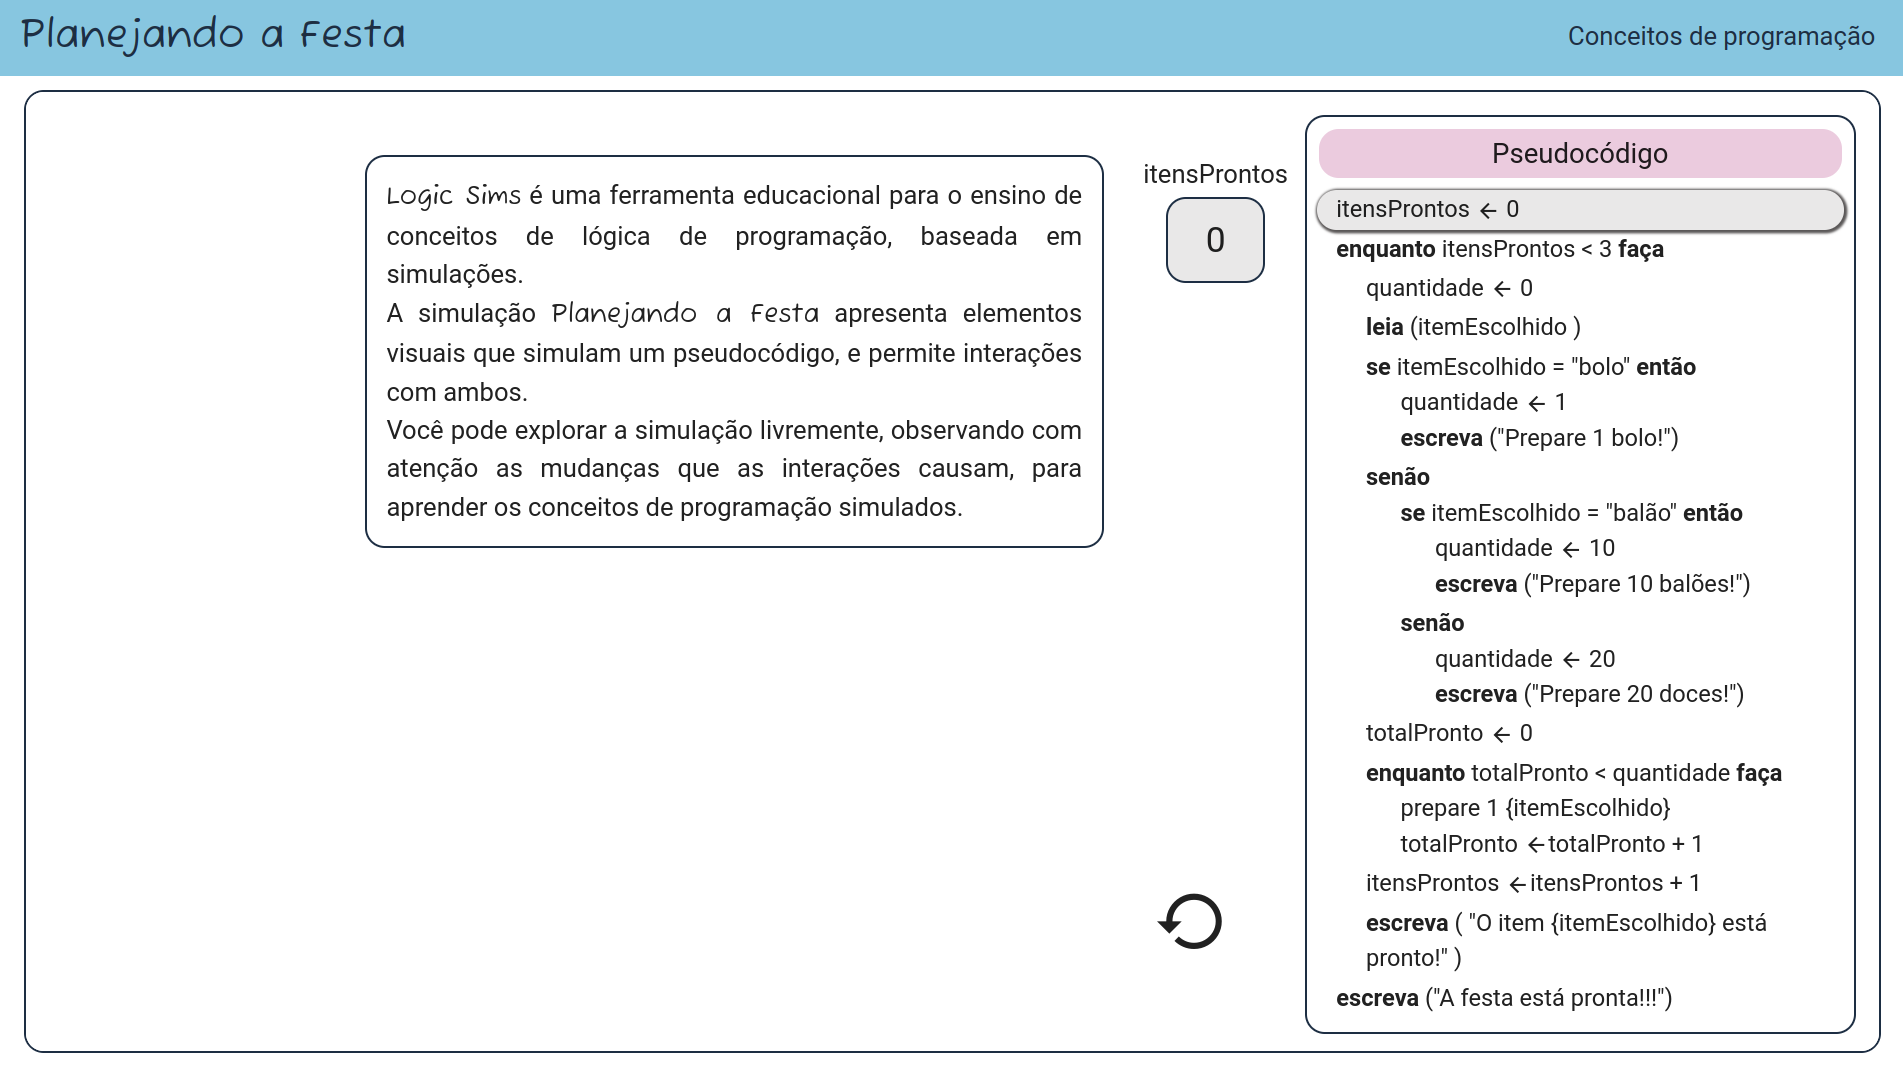
\includegraphics[scale=0.25]{tela_inicial_mvp.png}}
%     \caption{Tela inicial do MVP da simulação \enquote{Planejando a Festa}.}
%     \label{figure:tela_inicial}
% \end{figure}

% Nessa tela, é possível visualizar algumas das alterações sugeridas na etapa anterior. Essa nova versão da simulação também permite interações com o pseudocódigo, o qual tem as linhas destacadas com uma borda com uma animação que pisca quando é necessário interagir com ela. Esse recurso foi implementado para facilitar a visualização da \enquote{execução} de cada passo do pseudocódigo, o qual foi modificado. Adicionamos à lógica da simulação um laço de repetição externo para realizar a iteração na preparação dos três itens disponíveis para compor a festa, que faltava no projeto do protótipo.

% Assim, esta simulação permite selecionar três itens em quantidades distintas e preparar cada um até atingir as quantidades correspondentes até que a festa esteja pronta. A seleção de um item pelo usuário representa a entrada ou leitura de um valor no pseudocódigo, que condiciona a quantidade de itens a serem preparados. Ao escolher um item ou finalizar o seu preparo e quando a festa está pronta são impressas mensagens na tela em uma janela representando a saída de dados no pseudocódigo, como mostra a Figura \ref{figure:saida}. 

% \begin{figure}[h!]
%     \centering
%     \setlength{\fboxrule}{0.1pt} % espessura da borda da figura
%     \fbox{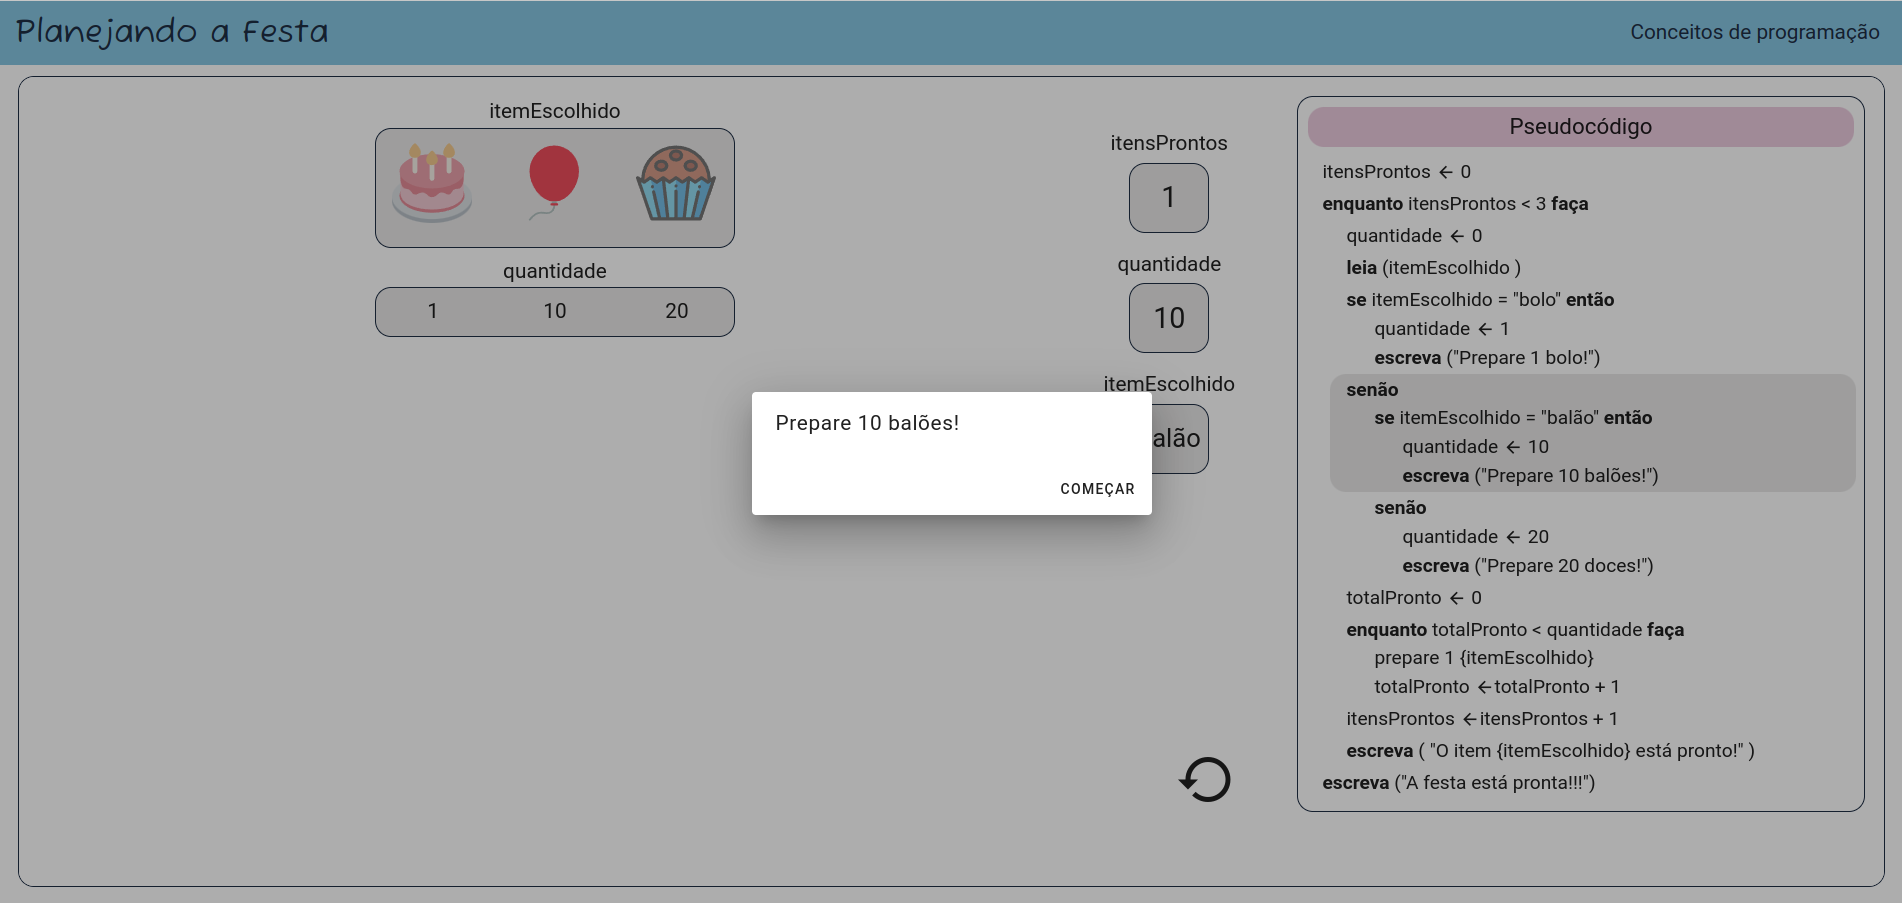
\includegraphics[scale=0.25]{saida.png}}
%     \caption{Representação visual do conceito de saída com a mensagem \enquote{impressa} na tela.}
%     \label{figure:saida}
% \end{figure}

% Ao selecionar um item para preparo, desabilitamos a escolha dos demais para que a interação com a simulação siga o fluxo do pseudocódigo e não permita que o usuário troque de item enquanto está dentro do laço de repetição interno, por exemplo. A Figura \ref{figure:item_escolhido} mostra o cenário em que o item \enquote{bolo} foi selecionado e os demais estão sombreados, não sendo possível clicar neles. Ainda, após o preparo de cada item, este fica desabilitado para escolha na iteração seguinte, limitando o preparo dos três itens (em qualquer ordem) para finalizar o preparo da festa e a simulação.

% \begin{figure}[h!]
%     \centering
%     \setlength{\fboxrule}{0.1pt} % espessura da borda da figura
%     \fbox{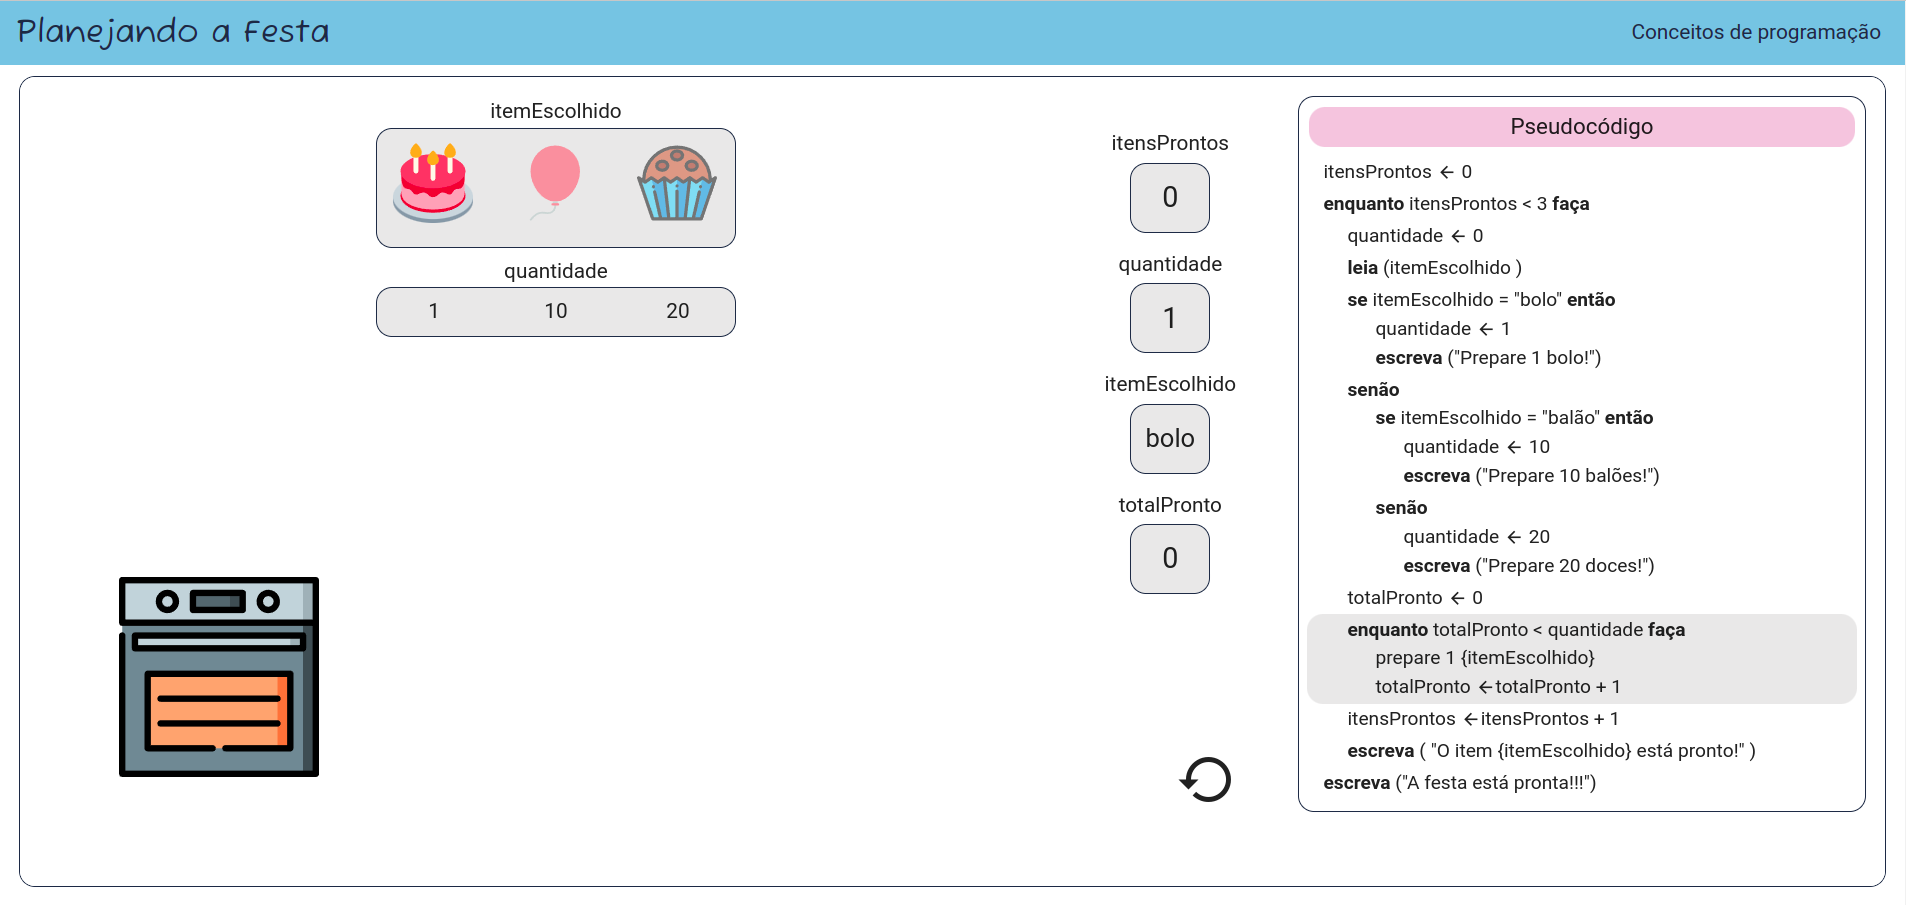
\includegraphics[scale=0.25]{item_escolhido.png}}
%     \caption{Escolhendo um item na simulação \enquote{Planejando a Festa}.}
%     \label{figure:item_escolhido}
% \end{figure}

% Na Figura \ref{figure:item_escolhido} também podemos observar que cada variável está separada em um elemento visual próprio. Além disso, removemos o controle do incremento do contador que indica a quantidade total pronta de cada item, deixando essa interação apenas nas figuras de preparo de cada item (fogão, cilindro de gás e pratos) para representar o laço de repetição interno do pseudocódigo. Ainda, adicionamos o pseudocódigo para a execução das atividades de preparo do item escolhido dentro desse laço.

% Outro recurso incorporado no pseudocódigo da simulação foi a adição de cores para diferenciar os conceitos de lógica de programação, o qual é comumente utilizado nas linguagens de programação em blocos. A escolha das cores foi feita através da ferramenta Coolors\footnote{\url{coolors.co}} que além de apresentar um gerador de paleta de cores, também disponibiliza um verificador de contraste. Ela segue as Diretrizes de Acessibilidade para Conteúdo Web (Web Content Accessibility Guidelines - WCAG), a qual define uma série de recomendações para tornar a web mais acessível \citep{caldwell2008web}. A categorização das cores foi feita da seguinte forma:

% \definecolor{variables}{HTML}{F9F1A8}
% \definecolor{inputOutput}{HTML}{FFC17C}
% \definecolor{operators}{HTML}{D0F4DE}
% \definecolor{conditional}{HTML}{E4C1F9}
% \definecolor{loop}{HTML}{A9DEF9}

% \begin{itemize}
%     \item \tcbox[on line,boxsep=0pt,left=2pt,right=2pt,top=2pt,bottom=2pt,colback=variables,colframe=variables]{Variáveis} (amarelo)
%     \item \tcbox[on line,boxsep=0pt,left=2pt,right=2pt,top=2pt,bottom=2pt,colback=inputOutput,colframe=inputOutput]{Entrada} e \tcbox[on line,boxsep=0pt,left=2pt,right=2pt,top=2pt,bottom=2pt,colback=inputOutput,colframe=inputOutput]{saída} (laranja)
%     \item \tcbox[on line,boxsep=0pt,left=2pt,right=2pt,top=2pt,bottom=2pt,colback=operators,colframe=operators]{Operadores} (verde)
%     \item \tcbox[on line,boxsep=0pt,left=2pt,right=2pt,top=2pt,bottom=2pt,colback=conditional,colframe=conditional]{Condicionais} (roxo)
%     \item \tcbox[on line,boxsep=0pt,left=2pt,right=2pt,top=2pt,bottom=2pt,colback=loop,colframe=loop]{Laço de repetição} (azul)
% \end{itemize}

% \noindent Além disso, indicamos o nome de cada conceito de lógica de programação. Esses recursos podem ser visualizados ao passar o mouse em cima de cada conceito. A Figura \ref{figure:pseudocodigo_destaque} apresenta as alterações destacadas.

% \begin{figure}[h!]
%     \centering
%     \setlength{\fboxrule}{0.1pt} % espessura da borda da figura
%     \fbox{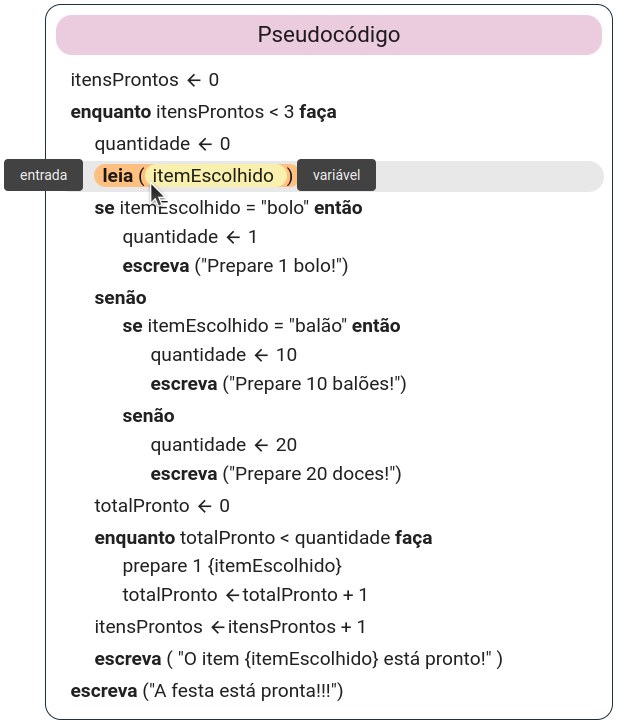
\includegraphics[scale=0.35]{pseudocodigo_destaque1.png}
%     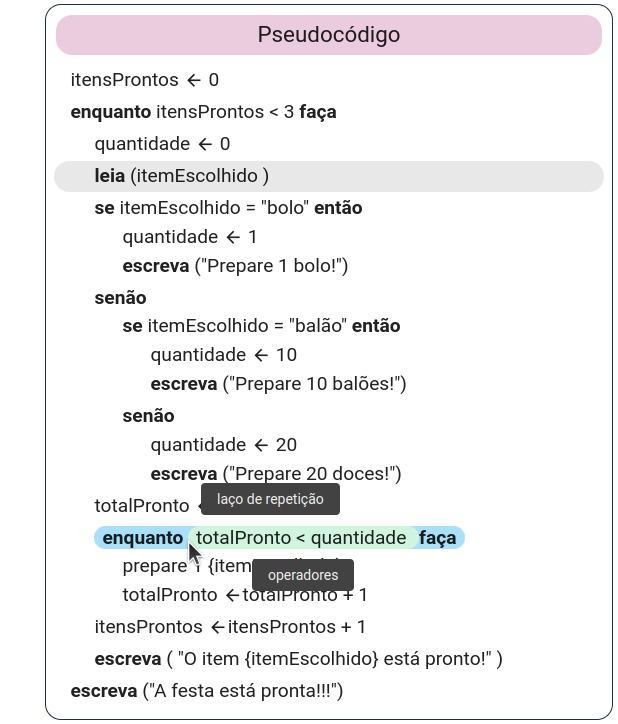
\includegraphics[scale=0.35]{pseudocodigo_destaque2.png}}
%     \caption{Destaques do pseudocódigo da simulação \enquote{Planejando a Festa} mostrando a separação em cores por conceito de lógica de programação e a indicação do nome deles ao passar o mouse por cima de cada um.}
%     \label{figure:pseudocodigo_destaque}
% \end{figure}

% Por fim, o link para \enquote{Ajuda} na barra de navegação foi renomeado para \enquote{Conceitos de programação} e ele abre uma caixa de diálogo contendo definições de cada conceito, com figuras e exemplos (Figura \ref{figure:conceitos_programacao}). As definições contêm pseudocódigos de exemplo que seguem o esquema de cores descrito acima.

% \begin{figure}[h!]
%     \centering
%     \setlength{\fboxrule}{0.1pt} % espessura da borda da figura
%     \fbox{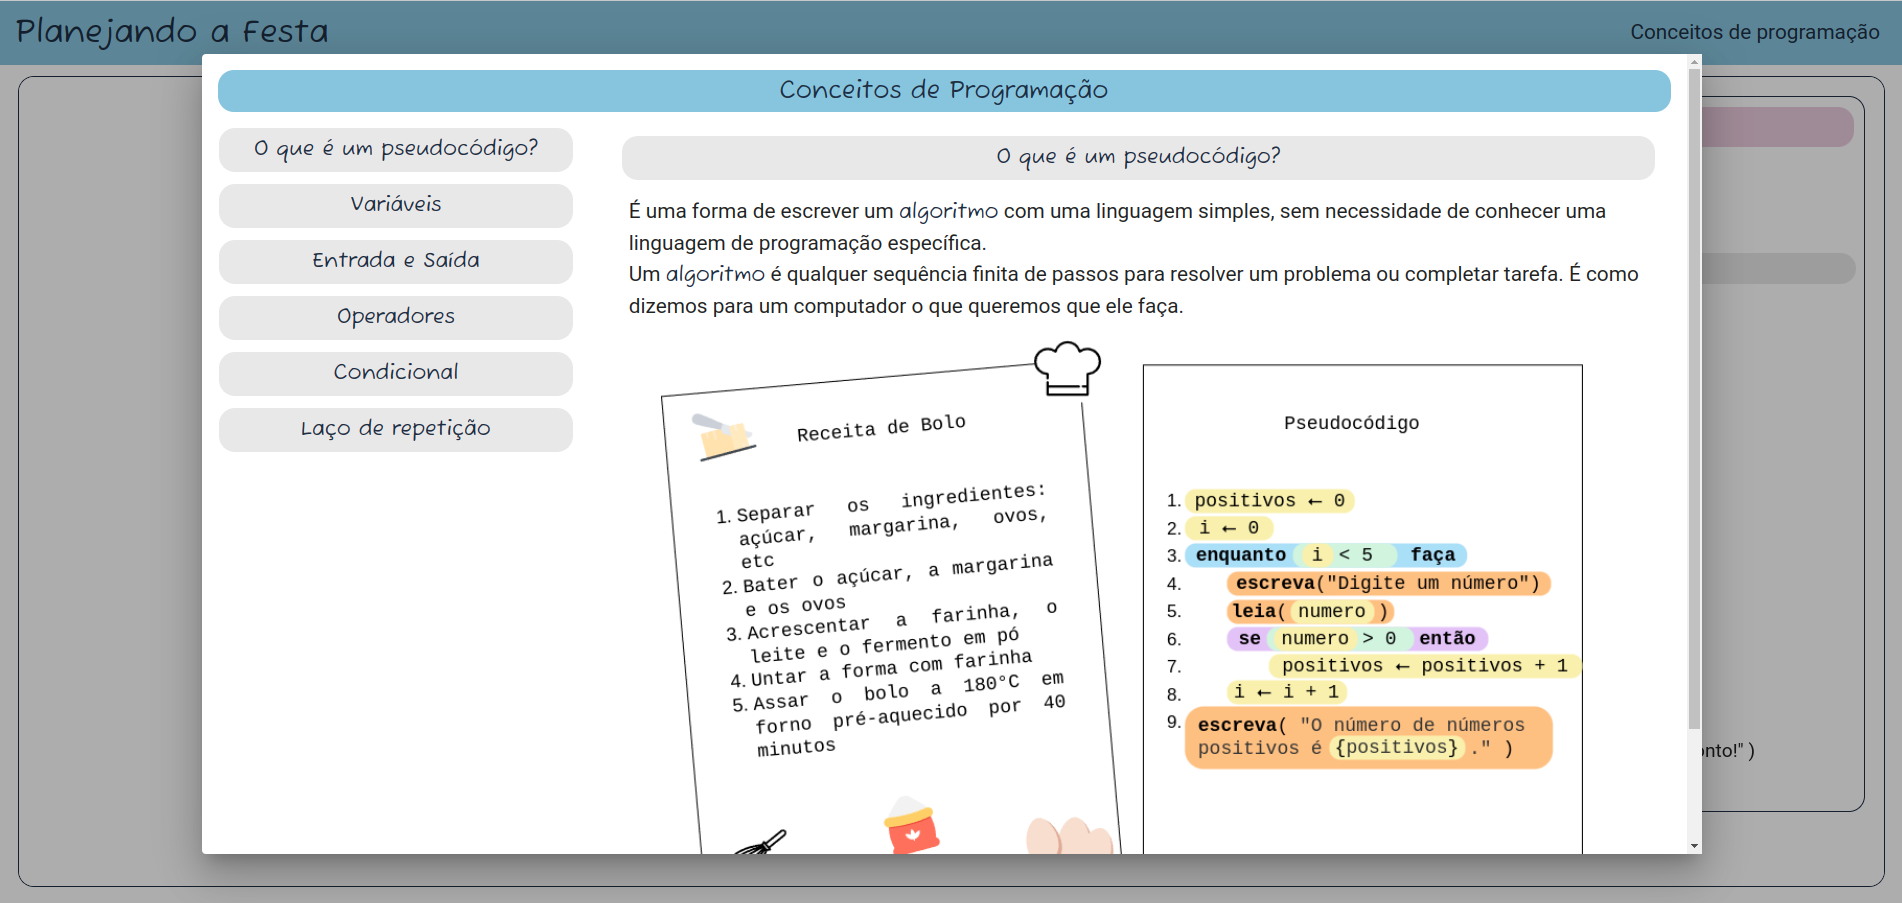
\includegraphics[scale=0.25]{conceitos_programacao.png}}
%     \caption{Caixa de diálogo contendo as definições dos conceitos de lógica de programação abordados na simulação \enquote{Planejando a Festa}. O menu lateral permite a escolha de um conceito, mostrando a sua definição e exemplos ao lado.}
%     \label{figure:conceitos_programacao}
% \end{figure}
%%%%%%%%%%%%%%%%%%%%%%%%%%%%%%%%%%%%%%%%%%%%%%%%%%%%%%%%%%%%%%%%%%%%%%%%%%%%%%%%

Assim, com o artefato implementado, criamos uma página para disponibilizar o MVP, através da ferramenta de versionamento de códigos GiHub, para a aplicação e avaliação da ferramenta em sala de aula.

\subsection{Avaliação do MVP}
% avaliação do sucesso do tratamento
A avaliação do MPV foi realizada utilizando um formulário de usabilidade e uma atividade para verificação do aprendizado dos conceitos de lógica de programação. Primeiramente, por meio do questionário de usabilidade, métrica comum na avaliação de um protótipo ou sistema, o MVP foi analisado considerando a facilidade de uso, de aprendizado e satisfação. Em particular, utilizamos o questionário SUS (\textit{System Usability Scale}), aplicado aos usuários finais.

%%%%%%%%%%%%%%%%%%%%%%%%%%%%%%%%%%%%%%%%%%%%%%%%%%%%%%%%%%%%%%%%%%%%%%%%%%%%%%%%
% Para isso, realizamos uma atividade com a duração de uma aula de 50 minutos com uma turma de 26 alunos, entre 13 e 14 anos, do 8° ano do Ensino Fundamental II da Escola de Aplicação da Faculdade de Educação da USP (FEUSP). Durante a aula, contamos com o apoio do professor Henri Silva, que leciona matemática para a turma. 

% A atividade realizada em aula foi dividade em três partes: na primeira, apresentamos um exemplo de pseudocódigo e código em Python de um programa que, dados cinco números de entrada, calcula a quantidade de números pares e de números ímpares; na segunda parte, os alunos exploraram o MVP com a simulação de forma livre; e na terceira, eles preencheram dois formulários, o de usabilidade e o da atividade de aprendizado, nessa ordem.
%%%%%%%%%%%%%%%%%%%%%%%%%%%%%%%%%%%%%%%%%%%%%%%%%%%%%%%%%%%%%%%%%%%%%%%%%%%%%%%%

Apesar de não haver medidas absolutas de usabilidade, é possível utilizar escalas gerais para comparar usabilidade em determinados contextos. O SUS representa uma escala de usabilidade com 10 itens que pode ser utilizada para avaliar sistemas \citep{brooke1996sus}. Ele é baseado na escala Likert, a qual contém afirmações e os avaliadores indicam o grau de acordo ou desacordo com cada uma, que varia de 1 a 5. Recomenda-se que as respostas para cada item sejam registradas de imediato, sem que os respondentes levem muito tempo pensando nelas.

Para obter o \textit{score} de usabilidade do sistema a partir do questionário SUS, primeiramente, a contribuição de cada item é normalizada para uma escala de 0 a 4. Em seguida, a soma das pontuações dos itens é multiplicada por 2.5, obtendo um \textit{score} em uma escala de 0 a 100. Entretanto, os autores não revelaram como analisar esta pontuação.

\citet{bangor2008empirical, bangor2009determining} realizaram um estudo onde avaliaram a usabilidade de diversos produtos e serviços utilizando o questionário SUS. Eles analisaram a média de pontuação do SUS em 273 estudos com cerca de 3500 pesquisas individuais. Os autores realizaram uma interpretação dessa pontuação, comparando os quartis dos \textit{scores}. Além disso, eles adicionaram uma afirmação ao questionário para avaliar a usabilidade do sistema através de uma escala de classificação de adjetivos, obtendo uma correlação entre eles e a média das pontuações. As médias que correspondem a cada adjetivo são as seguintes:

\begin{enumerate}
    \item pior imaginável (\textit{worst imaginable}): 12.5
    \item horrível (\textit{awful}) : 20.3
    \item ruim (\textit{poor}): 35.7
    \item ok (\textit{ok}): 50.9
    \item bom (\textit{good}): 71.4
    \item excelente (\textit{excellent}): 85.5
    \item melhor imaginável (\textit{best imaginable}): 90.9
\end{enumerate}

Os autores ainda expressaram preocupações com o uso do adjetivo \enquote{ok}, uma vez que ele sugere uma experiência aceitável com o sistema, enquanto a média de pontuações na faixa dele sugere deficiências. Eles acreditam que o termo \enquote{razoável} (\textit{fair}) seria melhor indicativo da usabilidade percebida pelos usuários.

Ademais, o SUS é considerado um questionário robusto e confiável, tendo sido utilizado em diversos projetos de pesquisa e avaliações na indústria \citep{brooke1996sus}. Embora não tenha sido projetado considerando necessidades específicas de compreensão por crianças, o questionário tem sido utilizado em vários estudos de testes e avaliações de ferramentas com crianças de diversas faixas etárias com sucesso \citep[i.e.][]{wronska2015ipad, dexheimer2017usability, sanchez2020usability, tasfia2023evaluating}. 

\citet{putnam2020adaptation} realizaram uma adaptação e teste do SUS com crianças na faixa etária de 7 a 11 anos. Os autores adaptaram o questionário, com o auxílio de professores da educação básica, em um contexto de aplicativos móveis de jogos focados no ensino de programação e pensamento computacional. As afirmações foram ainda modificadas pensando na separação de dois grupos de faixa etária, entre 7 e 8 anos e entre 9 e 11 anos. A Tabela \ref{table:sus} mostra os enunciados do SUS original e as adaptações propostas para os dois grupos mencionados, em inglês.

\begin{table}[h!]
\centering
\resizebox{\textwidth}{!}{%
\begin{tabular}{|c|c|c|c|}
\hline
\textbf{Afirmativa} & \textbf{SUS original}                                                                                                                 & \textbf{SUS adaptado: Grupo 9-11 anos}                                                                                                   & \textbf{SUS adaptado: Grupo 7-8 anos}                          \\ \hline
\textbf{1}           & \begin{tabular}[c]{@{}c@{}}I think that I would like to use this\\ system frequently.\end{tabular}                                    & \begin{tabular}[c]{@{}c@{}}If I had this {[}app{]} on my iPad, \\ I think that I would like to play it a lot.\end{tabular} & I would like to play {[}app{]} a lot more.       \\ \hline
\textbf{2}           & I found the system unnecessary complex.                                                                                               & \begin{tabular}[c]{@{}c@{}}I was confused many times \\ when I was playing {[}app{]}.\end{tabular}                         & {[}app{]} was hard to play.                      \\ \hline
\textbf{3}           & I thought the system was easy to use.                                                                                                 & I thought {[}app{]} was easy to use.                                                                                       & I thought {[}app{]} was easy to use.             \\ \hline
\textbf{4}           & \begin{tabular}[c]{@{}c@{}}I think that I would need the support of a\\  technical person to be able to use this system.\end{tabular} & \begin{tabular}[c]{@{}c@{}}I would need help from an\\  adult to continue to play {[}app{]}.\end{tabular}                  & I would need help to play {[}app{]} more.        \\ \hline
\textbf{5}           & \begin{tabular}[c]{@{}c@{}}I found the various functions in this\\ system were well integrated.\end{tabular}                          & \begin{tabular}[c]{@{}c@{}}I always felt like I knew what to do\\  next when I played {[}app{]}.\end{tabular}              & I knew what to do next when I played {[}app{]}.  \\ \hline
\textbf{6}           & \begin{tabular}[c]{@{}c@{}}I thought there was too much\\ inconsistency in the system.\end{tabular}                                   & \begin{tabular}[c]{@{}c@{}}Some of the things I had to do when\\  playing {[}app{]} did not make sense.\end{tabular}       & Some things in {[}app{]} made no sense.          \\ \hline
\textbf{7}           & \begin{tabular}[c]{@{}c@{}}I would imagine that most people would\\ learn to use this system very quickly.\end{tabular}               & \begin{tabular}[c]{@{}c@{}}I think most of my friends could\\  learn to play {[}app{]} very quickly.\end{tabular}          & {[}app{]} would be easy for my friends to learn. \\ \hline
\textbf{8}           & I felt the system was cumbersome to use.                                                                                              & \begin{tabular}[c]{@{}c@{}}Some of the things I had to do \\ to play {[}app{]} were kind of weird.\end{tabular}            & To play {[}app{]} I had to do some weird things. \\ \hline
\textbf{9}           & I felt very confident using the system.                                                                                               & I was confident when I was playing {[}app{]}.                                                                              & I was proud of how I played {[}app{]}.           \\ \hline
\textbf{10}          & \begin{tabular}[c]{@{}c@{}}I needed to learn a lot of things before\\ I could get going with this system.\end{tabular}                & \begin{tabular}[c]{@{}c@{}}I had to learn a lot of things \\ before playing {[}app{]} well.\end{tabular}                   & There was a lot to learn to play {[}app{]}.      \\ \hline
\end{tabular}%
}
\caption{Afirmativas em inglês do questionário de avaliação de usabilidade de sistemas SUS e adaptações propostas por \citet{putnam2020adaptation} para crianças entre 7 e 11 anos, dividida nos dois grupos.}
\label{table:sus}
\end{table} 

Além das simplificações das afirmações, os autores também utilizaram uma representação visual da escala de Likert (Figura \ref{figure:likert}), sugerida pelos docentes participantes do experimento.

\begin{figure}[h!]
    \centering
    \setlength{\fboxrule}{0.1pt} % espessura da borda da figura
    \fbox{\includegraphics[scale=0.5]{escalaLikertVisual.png}}
    \caption{Representação visual da escala de Likert \citep{putnam2020adaptation}.}
    \label{figure:likert}
\end{figure}

Os resultados obtidos nos experimentos mostraram que o questionário modificado juntamente com a escala visual foi compreendido pelas crianças participantes, necessitando apenas de clarificações mínimas. Eles ainda sugeriram alterações nas afirmações 6, 8 e 10 para melhorar a compreensão e a confiabilidade delas.

Dessa forma, utilizamos uma adaptação do questionário SUS para obter o \textit{feedback} dos estudantes sobre o MVP para avaliá-lo em relação a sua usabilidade. 

%%%%%%%%%%%%%%%%%%%%%%%%%%%%%%%%%%%%%%%%%%%%%%%%%%%%%%%%%%%%%%%%%%%%%%%%%%%%%%%%
% As 10 afirmações adaptadas do SUS e traduzidas para o português, apresentadas no formulário, estão enumeradas a seguir e a escala visual utilizada pode ser observada na Figura \ref{figure:likert_forms}.

% \begin{enumerate}
%     \item Eu gostaria de explorar mais a simulação.
%     \item Eu fiquei confuso(a) muitas vezes enquanto explorava a simulação.
%     \item Eu achei que a simulação foi fácil de usar.
%     \item Eu precisaria de ajuda para conseguir explorar a simulação.
%     \item Eu sabia o que era preciso fazer quando explorei a simulação.
%     \item Algumas coisas que eu tive que fazer enquanto explorava a simulação não fizeram sentido.
%     \item Eu acho que a maioria dos meus amigos podem aprender a usar a simulação muito rápido.
%     \item Algumas das coisas que eu tive que fazer para explorar a simulação foram estranhas.
%     \item Eu me senti confiante enquanto explorava a simulação.
%     \item Eu tive que aprender muitas coisas antes de explorar a simulação.
% \end{enumerate}

% \begin{figure}[h!]
%     \centering
%     \setlength{\fboxrule}{0.1pt} % espessura da borda da figura
%     \fbox{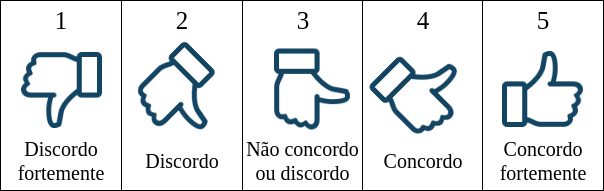
\includegraphics[scale=0.5]{escalaLikertformulario.png}}
%     \caption{Representação visual da escala de Likert utilizada no formulário de usabilidade.}
%     \label{figure:likert_forms}
% \end{figure}

% Ainda, ao final do formulário foram feitas duas perguntas dissertativas sobre o que o usuário mais gostou na simulação e o que menos gostou, além de um espaço adicional para deixar quaisquer comentários ou sugestões sobre ela.
%%%%%%%%%%%%%%%%%%%%%%%%%%%%%%%%%%%%%%%%%%%%%%%%%%%%%%%%%%%%%%%%%%%%%%%%%%%%%%%%

Ademais, através da atividade de aprendizado dos conceitos de programação, analisamos o potencial do ensino de computação utilizando simulações interativas. No Capítulo \ref{evaluation}, descrevemos a atividade realizada em sala de aula com a aplicação dos dois formulários para avaliação do artefato implementado.

%%%%%%%%%%%%%%%%%%%%%%%%%%%%%%%%%%%%%%%%%%%%%%%%%%%%%%%%%%%%%%%%%%%%%%%%%%%%%%%%
% A atividade foi dividida em duas partes com 6 perguntas cada. Em cada pergunta, era apresentada um trecho do pseudocódigo com um ou mais conceitos de lógica de programação e era pedido para selecionar a opção que melhor representasse aquele pedaço de pseudocódigo, entre as seguintes opções: variáveis, entrada, saída, operadores, condicional e laço de repetição. A primeira parte da atividade continha perguntas sobre ao pseudocódigo da simulação \enquote{Planejando a Festa}, explorada pelos estudantes. A segunda era referente à simulação \enquote{Guardando os Brinquedos}, a qual foi apresentada no formulário, para fornecer contexto para as questões, por meio de uma imagem (Figura \ref{figure:brinquedos_forms}). Esse protótipo foi modificado do projeto dos artefatos, apresentado na Seção \ref{validation}.

% \begin{figure}[h!]
%     \centering
%     \setlength{\fboxrule}{0.1pt} % espessura da borda da figura
%     \fbox{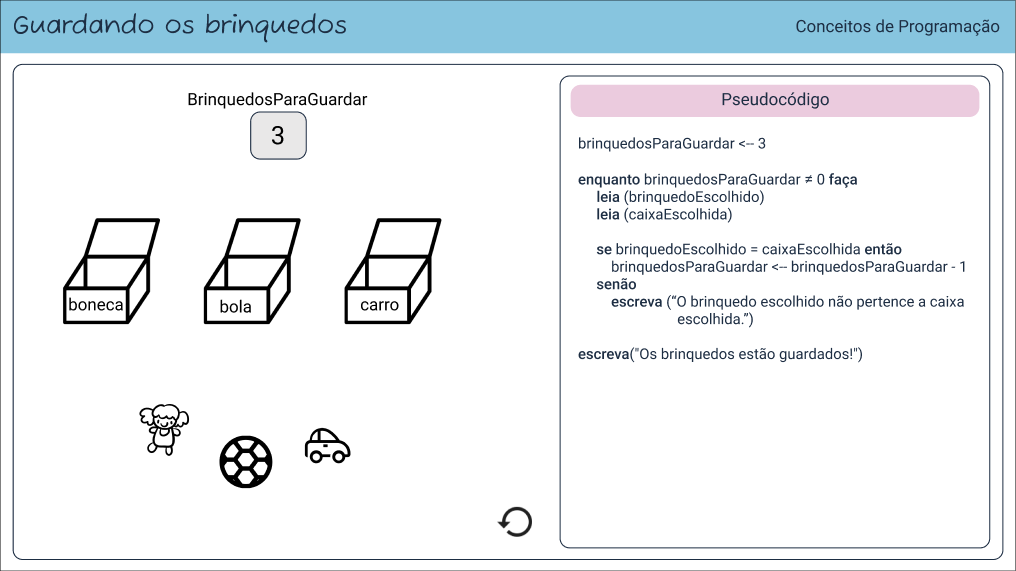
\includegraphics[scale=0.45]{prototipo_brinquedos_formulario.png}}
%     \caption{Protótipo da simulação \enquote{Guardando os Brinquedos} apresentado na atividade de aprendizado para fornecer contexto para as questões.}
%     \label{figure:brinquedos_forms}
% \end{figure}

% A Seção a seguir apresenta os resultados da avaliação do MVP feita a partir das respostas dos formulários.
%%%%%%%%%%%%%%%%%%%%%%%%%%%%%%%%%%%%%%%%%%%%%%%%%%%%%%%%%%%%%%%%%%%%%%%%%%%%%%%%